\begin{tabu}[t]{||c|c|c|c|c|c|c|c|c|c|c||}
	\hline
		\multicolumn{11}{||c||}{\textbf{Таблица квадратов}} \\
	\hline
		$a^2$ & \bf 0 & \bf 1 & \bf 2 & \bf 3 & \bf 4 & \bf 5 & \bf 6 & \bf 7 & \bf 8 & \bf 9 \\
	\hline
		\bf 10 & 100 & 121 & 144 & 169 & 196 & 225 & 256 & 289 & 324 & 361 \\
	\hline
		\bf 20 & 400 & 441 & 484 & 529 & 576 & 625 & 676 & 729 & 784 & 841 \\
	\hline
		\bf 30 & 900 & 961 & 1024 & 1089 & 1156 & 1225 & 1296 & 1369 & 1444 & 1521 \\
	\hline
		\bf 40 & 1600 & 1681 & 1764 & 1849 & 1936 & 2025 & 2116 & 2209 & 2304 & 2401 \\
	\hline
		\bf 50 & 2500 & 2601 & 2704 & 2809 & 2916 & 3025 & 3136 & 3249 & 3364 & 3481 \\
	\hline
		\bf 60 & 3600 & 3721 & 3844 & 3969 & 4096 & 4225 & 4356 & 4489 & 4624 & 4761 \\
	\hline
		\bf 70 & 4900 & 5041 & 5184 & 5329 & 5476 & 5625 & 5776 & 5929 & 6084 & 6241 \\
	\hline
		\bf 80 & 6400 & 6561 & 6724 & 6889 & 7056 & 7225 & 7396 & 7569 & 7744 & 7921 \\
	\hline
		\bf 90 & 8100 & 8281 & 8464 & 8649 & 8836 & 9025 & 9216 & 9409 & 9604 & 9801 \\
	\hline
		\bf 100 & 10000 & 10201 & 10404 & 10609 & 10816 & 11025 & 11236 & 11449 & 11664 & 11881 \\
	\hline
\end{tabu}

\begin{tabu}[t]{||c|c|c|c|c|c|c||}
	\hline
		\multicolumn{7}{||c||}{\textbf{Таблица степеней}} \\
	\hline
		$a^n$ & \bf 2 & \bf 3 & \bf 4 & \bf 5 & \bf 6 & \bf 7 \\
	\hline
		\bf 2 & 4 & 8 & 16 & 32 & 64 & 128 \\
	\hline
		\bf 3 & 9 & 27 & 81 & 243 & 729 & 2187 \\
	\hline
		\bf 4 & 16 & 64 & 256 & 1024 & 4096 & 16384 \\
	\hline
		\bf 5 & 25 & 125 & 625 & 3125 & 15625 & 78125 \\
	\hline
		\bf 6 & 36 & 216 & 1296 & 7776 & 46656 & 279936 \\
	\hline
		\bf 7 & 49 & 343 & 2401 & 16807 & 117649 & 823543 \\
	\hline
		\bf 8 & 64 & 512 & 4096 & 32768 & 262144 & 2097152 \\
	\hline
		\bf 9 & 81 & 729 & 6561 & 59049 & 531441 & 4782969 \\
	\hline
\end{tabu}

\begin{tabu}[t]{||c||c|c||}
	\hline
		\multicolumn{3}{||c||}{\textbf{Формулы сокращенного умножения}} \\
	\hline
	\hline
		\multirow{2}{*}{\bf 2}&
		$ a^2-b^2 = (a-b)(a+b) $ &
		$ a^2 + b^2 = (a + b)^2 - 2ab $ \\		
	\cline{2-3}
		&
		$ (a\pm b)^2 = a^2 \pm 2ab + b^2 $ &
		$ (a + b + c)^2 = a^2 + b^2 + c^2 + 2ab + 2ac + 2bc $ \\		
	\hline
	\hline
		\multirow{2}{*}{\bf 3}&
		$ a^3 \pm b^3 = (a\pm b)(a^2 \mp ab + b^2) $ &
		$ (a \pm b)^3 = a^3 \pm 3a^2b + 3ab^2 \pm b^3 $ \\
	\cline{2-3}
		&
		\multicolumn{2}{c||}{$ (a + b + c)^3 = a^3 + b^3 + c^3 + 3a^2b + 3a^2c + 3ab^2 + 3ac^2 + 3b^2c + 3bc^2 + 6abc $} \\		
	\hline
	\hline
		\multirow{2}{*}{\bf 4}&
		\multicolumn{2}{c||}{$ a^4 - b^4 = (a^2 - b^2)(a^2 + b^2) = (a-b)(a^3-a^2b+ab^2-b^3) $} \\
	\cline{2-3}
		&
		$ a^4 + a^2 + 1 = (a^2 - a + 1)(a^2 - a + 1) $ &
		$ (a\pm b)^4 = a^4 \pm 4a^3b + 6a^2b^2 \pm 4ab^3 + b^4 $ \\
	\hline
	\hline
		\multirow{3}{*}{\bf n}&
		\multicolumn{2}{c||}{$ a^n - b^n = (a-b)(a^{n-1}+a^{n-2}b + a^{n-3}b^2 + \ldots + a^2b^{n-3} + ab^{n-2} + b^{n-1}) $} \\
	\cline{2-3}
		&
		\multicolumn{2}{c||}{$ a^n + b^n = (a+b)(a^{n-1}-a^{n-2}b + a^{n-3}b^2 - \ldots + a^2b^{n-3} - ab^{n-2} + b^{n-1}),\quad n - \text{нечетное} $} \\
	\cline{2-3}
		&
		$ (a-b)^{2n} = (b-a)^{2n} $ &
		$ (a-b)^{2n+1} = -(b-a)^{2n+1} $ \\
	\hline
\end{tabu}

\begin{tabu}[t]{||c|c||}
	\hline
		\multicolumn{2}{||c||}{\textbf{Квадратное уравнение}} \\
	\hline
	\hline
		\specialcell{
			$\displaystyle a\, x^2 + b\, x + c = 0 $ \\ 
			$\displaystyle a\, (x - x_1)\, (x - x_2) = 0 $ \\ 
			$\displaystyle x_{1/2} = \frac{-b\pm \sqrt{\mathstrut b^2-4ac}}{2\, a} $
		} &
		$\displaystyle \left\{ \begin{aligned}
			& x_1-x_2 = -\frac{b}{a} \\
			& x_1 \cdot x_2 = \frac{c}{a}
		\end{aligned} \right. $ \\
	\hline
\end{tabu}

\begin{tabu}[t]{||c||}
	\hline
		\textbf{Выделение полного квадрата} \\
	\hline
		$\displaystyle ax^2 + bx + c = 0 $ \\
	\hline
		$\displaystyle a\left(x + \frac{b}{2a} \right)^2 + \frac{4ac-b^2}{4a} = 0 $ \\
	\hline
\end{tabu}

\begin{tabu}[t]{||c||}
	\hline
		\textbf{Симметричное уравнение} \\
	\hline
		$\displaystyle \left(x+\frac{1}{x}\right)^2 = \left(x^2+\frac{1}{x^2}\right) + 2 $ \\
	\hline
		\specialcell{
		$\displaystyle 3x^4 + 4x^3 - x^2 + 4x + 3 = 0 $ - делим на $x^2$ \\
		$\displaystyle 3\left(x^2 + \frac{1}{x^2}\right) + 4\left(x+\frac{1}{x}\right)-1 = 0 $ \\
		$\displaystyle 3y^2 + 4y + 5 = 0 $ \\
		} \\
	\hline
\end{tabu}

\begin{tabu}[t]{||ccccccc||}
	\hline
		\multicolumn{7}{||c||}{Если дано $n$ чисел $a_1$, $a_2$, $\ldots$, $a_n$, то действительны неравенства:}\\
	\hline
	\hline
		\specialcell{\textbf{Среднее} \\ \textbf{пропорциональное}} & & \specialcell{\textbf{Среднее} \\ \textbf{геометрическое}} & & \specialcell{\textbf{Среднее} \\ \textbf{арифметическое}} & & \specialcell{\textbf{Среднее} \\ \textbf{квадратичное}} \\
		$ \cfrac{n}{\cfrac{1}{a_1}+\cfrac{1}{a_2}+\ldots+\cfrac{1}{a_n}} $ & $ \leqslant $ & $ \sqrt[n]{a_1\, a_2\, \ldots\, a_n} $ &  $ \leqslant $ & $\cfrac{a_1+a_2+\ldots+a_n}{n}$ & $ \leqslant $ & $\sqrt{\cfrac{a_1^2+a_2^2+\ldots+a_n^2}{n}}$ \\
	\hline
\end{tabu}

$\displaystyle \sqrt{\mathstrut a\pm \sqrt{\mathstrut b}} = \sqrt{\mathstrut \frac{a + \sqrt{\mathstrut a^2 - b}}{2}}\pm \sqrt{\mathstrut \frac{a - \sqrt{\mathstrut a^2 - b}}{2}} $

$\displaystyle a_1 b_1 + a_2 b_2 \ldots + a_n b_n \leqslant \sqrt{a_1^2 + a_2^2 + \ldots + a_n^2}\cdot \sqrt{b_1^2 + b_2^2 + \ldots + b_n^2} $

\begin{tabu}[t]{ccccccc}
	Если $f(a) = 0$, $f'(x)>0$ при $x \in (a; +\infty)$, $f$ непрерывна в $a$, то: \\
	$f(\lambda b + (1-\lambda)a) \leqslant \lambda f(b) + (1-\lambda) f(a)$, $\lambda \in [0, 1]$
\end{tabu}

$\displaystyle (1+a)^b > 1 + ab $, при $a > 0$, $ b > 1 $.

$\displaystyle \sum_{n=0}^{\infty} a_n x^n \cdot \sum_{n=0}^{\infty} b_n x^n = \sum_{n=0}^{\infty} c_n x^n $

Произведение числовых рядов:

$\displaystyle c_n = a_n b_0 + a_{n-1} b_1 + \ldots + a_0 b_n = \sum_{k=0}^{n} a_{n-k} b_k $

$\displaystyle \sum^{n}_{k=1} \frac{1}{k} = 1 + \frac12 + \frac13 + \ldots + \frac{1}{n} = \gamma + \ln n + \varepsilon_n, \quad \lim_{n\to \infty} \varepsilon_n = 0, \quad \gamma \thickapprox 0.577215664 \ldots $

%--------------------------------------------------------------------------------%

\begin{tabu}{||c|c||}
	\hline
		\multicolumn{2}{||c||}{\textbf{НОД} и \textbf{НОК}} \\
	\hline
	\hline
		\multicolumn{2}{||c||}{$ \text{НОД}(a, b) = \gcd(a, b) = c $} \\
		\multicolumn{2}{||p{11cm}||}{
			\textbf{Наибольший Общий Делитель} от чисел $a$ и $b$ - это наибольшее возможное число $c$, такое, что $a$ и $b$ делятся на $c$ без остатка.
		} \\
		\multicolumn{2}{||p{11cm}||}{
			Если образовать дробь из чисел $a$ и $b$ то, чтобы сделать дробь несократимой, необходимо их оба разделить на $\displaystyle \gcd(a, b) $:
		} \\
		\multicolumn{2}{||c||}{$\displaystyle \frac{a}{b} = \frac{a}{\gcd(a, b)}:\frac{b}{\gcd(a, b)}$} \\
	\hline
	\hline
		\multicolumn{2}{||c||}{$ \text{НОК}(a, b) = \lcm(a, b) = c $} \\
		\multicolumn{2}{||p{11cm}||}{
			\textbf{Наименьшее Общее Кратное} от чисел $a$ и $b$  - это наименьшее возможное число $c$, такое, что $c$  делится и на $a$ и на $b$ без остатка. 
		} \\
		\multicolumn{2}{||p{11cm}||}{
			При сложении дробей образуется одна дробь, и нижняя  часть у нее НОК знаменателей:
		} \\
		\multicolumn{2}{||c||}{
			\specialcell{
				 $\displaystyle\frac{a}{b} + \frac{c}{d} = \frac{a\cdot \frac{\lcm(b, d)}{b} + c\cdot \frac{\lcm(b, d)}{d}}{\lcm(b, d)}$
			}
		} \\
	\hline
	\hline
		\specialcell{
			$\displaystyle \gcd(a, a) = a$ \\
			$\displaystyle \lcm(a, a) = a$ \\
		} &
		\specialcell{
			$\displaystyle \gcd(a, \gcd(b, c)) = \gcd(\gcd(a, b), c)$ \\
			$\displaystyle \lcm(a, \lcm(b, c)) = \lcm(\lcm(a, b), c)$ \\
		} \\
	\hline
		\specialcell{
			$\displaystyle \gcd(a, b) = \gcd(b, a)$ \\
			$\displaystyle \lcm(a, b) = \lcm(b, a)$ \\
		} &
		\specialcell{
			$\displaystyle \gcd(a, b, c) = \gcd(\gcd(a, b), c)$ \\
			$\displaystyle \lcm(a, b, c) = \lcm(\lcm(a, b), c)$ \\
		} \\
	\hline
		\multicolumn{2}{||c||}{\specialcell{
			$\displaystyle \gcd(a_0, a_1, \ldots, a_n) = \gcd(\gcd(a_0, a_1, \ldots, a_{n-1}), a_n)$ \\
			$\displaystyle \lcm(a_0, a_1, \ldots, a_n) = \lcm(\lcm(a_0, a_1, \ldots, a_{n-1}), a_n)$ \\
		}} \\
	\hline
		\specialcell{
			$\displaystyle \lcm(a, \gcd(a, b)) = a$ \\
			$\displaystyle \gcd(a, \lcm(a, b)) = a$ \\
		} &
		\specialcell{
			$\displaystyle \gcd(a + m\cdot b, b) = \gcd(a, b)$ \\
			$\displaystyle \gcd(c\cdot a, c\cdot b) = |c|\cdot\gcd(a, b)$ \\
		} \\
	\hline
		\multicolumn{2}{||c||}{\specialcell{
			$\displaystyle \gcd(a, \lcm(b, c)) = \lcm(\gcd(a, b), \gcd(a, c))$ \\
			$\displaystyle \lcm(a, \gcd(b, c)) = \gcd(\lcm(a, b), \lcm(a, c))$ \\
		}} \\
	\hline
		\specialcell{
			$\displaystyle \lcm(a, b) = \frac{|a\cdot b|}{\gcd(a, b)}$ \\
			$\displaystyle \gcd(a, 0)=|a|, a \neq 0$ \\
		} &
		\specialcell{
			\textbf{Алгоритм Евклида:} \\
			$\gcd(a, b) = \gcd(a, a \mod b), a > b$ \\
			$\gcd(a, 0)=|a|, a \neq 0$ \\
		} \\
	\hline
\end{tabu}

\begin{tabu}[t]{||c|c|c|c||}
	\hline
		\multicolumn{4}{||c||}{Модуль} \\
	\hline
	\hline
		\multicolumn{4}{||c||}{$\displaystyle |x| = \sqrt{x^2} = x \cdot \mathop{\text{sgn}} x = \max \{x, -x\} $} \\
	\hline
		$\displaystyle |a| \geqslant 0 $ &
		$\displaystyle |a| \geqslant a $ &
		$\displaystyle |a|^2 = a^2 $ &
		$\displaystyle |-a| = |a| $ \\
	\hline
		\multicolumn{2}{||c|}{$\displaystyle |ab| = |a|\cdot|b| $} &
		$\displaystyle \left|\frac{a}{b}\right| = \frac{|a|}{|b|} $ &
		$\displaystyle |a^k| = |a|^k $ \\
	\hline
		\multicolumn{2}{||c|}{\specialcell{
			$\displaystyle |a\pm b| \leqslant |a| + |b| $ \\
			$\displaystyle |a| - |b| \leqslant |a+b| $ \\
			$\displaystyle |a\pm b| \geqslant ||a| - |b|| $ \\
		}} &
		\multicolumn{2}{c||}{$\displaystyle |a| \Rightarrow \left[ \begin{aligned}
			& \left\{ \begin{aligned}
				& a \\
				& a \geqslant 0
			\end{aligned}\right. \\
			& \left\{ \begin{aligned}
				& -a \\
				& a < 0
			\end{aligned}\right.
		\end{aligned}\right. $} \\
	\hline
\end{tabu}

%--------------------------------------------------------------------------------%

\begin{tabu}[t]{||c||}
	\hline	
		\specialcell{\textbf{Свойства} \\ \textbf{степени}} \\
	\hline
		$\displaystyle a^m = \underbrace{a\, a \, \ldots \, a }_{m сомножителей} $ \\
	\hline
		$\displaystyle a^{-m} = \frac{1}{a^m} $ \\
	\hline
		$\displaystyle a^0 = 1 $ \\
	\hline
		$\displaystyle a^n\, a^m = a^{n+m} $ \\
	\hline
		$\displaystyle \frac{a^n}{a^m} = a^{n-m} $ \\
	\hline
		$\displaystyle (a^n)^m = a^{nm} $ \\
	\hline
		$\displaystyle (ab)^n = a^n\, b^n $ \\
	\hline
		$\displaystyle \left(\frac{a}{b} \right)^n = \frac{a^n}{b^n} $ \\
	\hline
		$\displaystyle a^{\frac{1}{n}} = \sqrt[n]{a} $ \\
	\hline
\end{tabu}



%--------------------------------------------------------------------------------%

\begin{tabu}[t]{||@{}c@{}|@{}c@{}||}
	\hline	
		\multicolumn{2}{||c||}{\textbf{Свойства корня}} \\
	\hline
		\begin{tabu}[t]{c}
				$\displaystyle \sqrt[n]{\mathstrut a\, b} = \sqrt[n]{\mathstrut a} \, \sqrt[n]{\mathstrut b} $ \\
			\hline
				$\displaystyle \sqrt[n]{\mathstrut \frac{a}{b}} = \frac{\sqrt[n]{\mathstrut a}}{\sqrt[n]{\mathstrut b}} $ \\
			\hline
				$\displaystyle (\sqrt[n]{\mathstrut a})^k = \sqrt[n]{\mathstrut a^k} = a^{\frac{k}{n}} $ \\
			\hline
				$\displaystyle \sqrt[2n + 1]{\mathstrut -a} = -\sqrt[2n + 1]{\mathstrut a} $ \\
			\hline
				$\displaystyle \sqrt[n]{\mathstrut \sqrt[k]{\mathstrut a}} = \sqrt[n\, k]{\mathstrut a} $ \\
			\hline
				$\displaystyle \sqrt[n]{\mathstrut a} = \sqrt[n\, k]{\mathstrut a^k} $ \\
			\hline
				$\displaystyle \sqrt[2n]{\mathstrut a^{2n}} = |a| $ \\
		\end{tabu} &
		\begin{tabu}[t]{c}
				$\displaystyle \sqrt{a} = b \Rightarrow  \left\{ \begin{aligned}
					& a = b^2 \\
					& b > 0
				\end{aligned}\right. $ \\
			\hline
				$\displaystyle \sqrt{a} = \sqrt{b} \Rightarrow  \left\{ \begin{aligned}
					& a = b \\
					& a > 0
				\end{aligned}\right. $ \\
			\hline
				$\displaystyle \sqrt{a} > b \Rightarrow  \left[ \begin{aligned}
					& \left\{ \begin{aligned}
						& a > b^2 \\
						& b \geqslant 0
					\end{aligned} \right. \\
					& \left\{ \begin{aligned}
						& b < 0 \\
						& a > 0
					\end{aligned} \right.
				\end{aligned} \right. $ \\
			\hline
				$\displaystyle \sqrt{a} < b \Rightarrow \left\{ \begin{aligned}
						& b > 0 \\
						& a < b^2
					\end{aligned} \right. $ \\
		\end{tabu} \\
	\hline
\end{tabu}



%--------------------------------------------------------------------------------%

\begin{tabu}{||@{}c@{}|c||}
	\hline
		\multicolumn{2}{||c||}{\textbf{Логарифм}} \\
	\hline
	\hline
		$\displaystyle a^x = b \Leftrightarrow \log_a b = x $ &
		\specialcell{
			ОДЗ: $\displaystyle \log_a b = c,$ \\
			$\displaystyle a > 0,\, a \neq 1,\, b > 0 $ \\
		} \\
	\hline
		$\displaystyle a^{\log_b c} = c^{\log_b a} $ &
		$\displaystyle \log_a (xy) = \log_a |x| + \log_a |y| $ \\
	\hline
		$\displaystyle \log_a b = \frac{\log_x b}{\log_x a} $ &
		$\displaystyle \log_a \frac{x}{y} = \log_a |x| - \log_a |y| $ \\
	\hline
		$\displaystyle \log_a \frac{1}{b} = -\log_a b $ &
		$\displaystyle \log_a b = \frac{1}{\log_b a} $ \\
	\hline
		\specialcell{
				$\displaystyle \,\, \log_{a^k} x^m = \frac{m}{k} \log_{|a|} |x| \,\, $ \\
			\hline
				$\displaystyle a^{\log_a x} = e^{\ln x} = x $ \\
			\hline
				$\displaystyle \log_3 9 = 2 $ \\
			\hline
				$\displaystyle \ln a = \log_e a $ \\
			\hline
				$\displaystyle \lg a = \log_{10} a $ \\
			\hline
				$\displaystyle \log_a 1 = 0 $ \\
			\hline
				$\displaystyle \log_a a = 1 $ \\
		} &
		\begin{tabu}{cc}
			\rotatebox[origin=c]{90}{$ \log_{\varphi(x)} f(x) \geqslant \log_{\varphi(x)} g(x) $}
			&
			$\displaystyle \Rightarrow \left[
			\begin{aligned}
				\left\{ \begin{aligned}
					& f(x) \geqslant g(x) \\
					& g(x) > 0 \\
					& \varphi(x) > 1
				\end{aligned} \right. & \\
				\left\{ \begin{aligned}
					& f(x) \leqslant g(x) \\
					& f(x) > 0 \\
					& \varphi(x) > 0 \\
					& \varphi(x) < 1
				\end{aligned} \right. & \\
			\end{aligned} \right. $\\
		\end{tabu} \\
	\hline
\end{tabu}

%--------------------------------------------------------------------------------%

\begin{tabu}[t]{||c|c|c|c|c|c|c||}
	\hline
		\multicolumn{7}{||c||}{\textbf{Основные понятия комбинаторики}} \\
	\hline
	\hline
		Обозначение &
		$\displaystyle A_n^m $ &
		$\displaystyle \widetilde{A}_n^m $ &
		$\displaystyle C_n^m $ &
		$\displaystyle \widetilde{C}_n^m $ &
		$\displaystyle P_n $ &
		$\displaystyle P(n_1, \ldots, n_k) $ \\
	\hline
		Формула &
		$\displaystyle \frac{n!}{(n-m)!} $ &
		$\displaystyle n^m $ &
		$\displaystyle \frac{n!}{m!(n-m)!} $ &
		$\displaystyle \frac{(n+m-1)!}{m!(n-1)!} $ &
		$\displaystyle n! $ &
		$\displaystyle \frac{(n_1 + \ldots + n_k)!}{n_1!n_2!\cdot\ldots\cdot n_k!} $ \\
	\hline
		Частный случай &
		$\displaystyle A_3^2 = 6 $ &
		$\displaystyle \widetilde{A}_3^2 = 9 $ &
		$\displaystyle C_3^2 = 3 $ &
		$\displaystyle \widetilde{C}_3^2 = 6 $ &
		$\displaystyle P_3 = 6 $ &
		$\displaystyle P(2, 2, 0) = 6 $ \\
	\hline
		\specialcell{Множество в \\ этом случае \\ $\displaystyle \{a, b, c\} \rightarrow $ ?} &
		$\displaystyle \begin{aligned}\{&ab, ac, ba, \\ &bc, ca, cb\} \end{aligned} $ &
		$\displaystyle \begin{aligned} \{ &aa, ab, ac, \\ &ba, bb, bc, \\ &ca, cb, cc\}\end{aligned} $ &
		$\displaystyle \{ab, ac, bc\} $ &
		$\displaystyle \begin{aligned} \{&aa, ab, ac, \\ &bb, bc, cc\} \end{aligned} $ &
		$\displaystyle \begin{aligned} \{&abc, acb, \\ &bac, bca, \\ &cab, cba\} \end{aligned} $ &
		$\displaystyle \begin{aligned} \{&aabb, abab, baab, \\ &baba, bbaa, abba\} \end{aligned} $ \\
	\hline
		\specialcell{Перестановки \\ различны?} &
		+ & + & -- & -- & + & + \\
	\hline
		Повторения? &
		-- & + & -- & + & -- & + \\
	\hline
\end{tabu}

\begin{tabu}[t]{||c|c||}
	\hline
		\multicolumn{2}{||c||}{\textbf{Формулы комбинаторики}} \\
	\hline
	\hline
		$\displaystyle C^m_n = {n\choose m} = \frac{A^m_n}{P_m} = C^{n-m}_n $ &
		$\displaystyle \widetilde{C}^m_n = C^m_{n+m-1} = C^{n-1}_{n+m-1} $ \\
	\hline
		$\displaystyle C^0_n + C^1_n + \ldots + C^n_n = 2^n $ &
		$\displaystyle C^m_n + C^{m+1}_n = C^{m+1}_{n+1} $ \\		
	\hline
		\multicolumn{2}{||c||}{$\displaystyle (a+b)^n = C^0_n\cdot a^n + C^1_n\cdot a^{n-1}b + \ldots + C^n_n\cdot b^n $} \\
	\hline
	\hline
		$\displaystyle (a+b)^n = T_1 + T_2 + \ldots + T_{n+1} $ &
		$\displaystyle T_{k} = C^{k-1}_n\cdot a^{n-k-1}b^{k-1} $ \\
	\hline
\end{tabu}

%--------------------------------------------------------------------------------%

\begin{tabu}[t]{||c|c||}
	\hline	
		\multicolumn{2}{||c||}{\textbf{Арифметическая прогрессия}} \\
	\hline
		\multicolumn{2}{||c||}{$\displaystyle a_1,\, a_2,\, a_3,\, \ldots ,\, a_n $ - ариф. прогрессия $ \Leftrightarrow $} \\
		\multicolumn{2}{||c||}{$\displaystyle a_1,\, a_1 + d,\, a_1 + 2d,\,  \ldots ,\, a_1 + (n-1)\cdot d $} \\
	\hline
		\multicolumn{2}{||c||}{$\displaystyle a_n = a_{n-1} + d = a_1 + (n-1)\cdot d $} \\
	\hline
		$\displaystyle d = \frac{a_n-a_m}{n-m}, n \neq m $ &
		$\displaystyle a_n = \frac{a_{n+1} + a_{n-1}}{2} $ \\
	\hline
		\multicolumn{2}{||c||}{$\displaystyle S_n = \sum_{k=1}^n  a_k = a_1 + a_2 + \ldots + a_n $} \\
	\hline
		$\displaystyle S_n = \frac{a_1 + a_n}{2}\cdot n $ &
		$\displaystyle S_n = \frac{2a_1 + d(n-1)}{2}\cdot n $ \\
	\hline
\end{tabu}

\begin{tabu}[t]{||c|c||}
	\hline	
		\multicolumn{2}{||c||}{\textbf{Геометрическая прогрессия}} \\
	\hline
		\multicolumn{2}{||c||}{$\displaystyle b_1,\, b_2,\, b_3,\, \ldots ,\, b_n $ - геом. прогрессия $\Leftrightarrow$} \\
		\multicolumn{2}{||c||}{$\displaystyle b_1,\, b_1 q,\, b_1 q^2,\,  \ldots ,\, b_1 q^{n-1} $} \\
	\hline
		\multicolumn{2}{||c||}{$\displaystyle b_n = b_{n-1}\cdot q = b_1 \cdot q^{n-1} $} \\
	\hline
		$\displaystyle q^{n-m} = \frac{b_n}{b_m} $ &
		$\displaystyle b_n = \sqrt{b_{n+1}\cdot b_{n-1}}, b_n \neq 0 $ \\
	\hline
		\multicolumn{2}{||c||}{$\displaystyle S_n = \sum_{k=1}^n  b_k = b_1 + b_2 + \ldots + b_n $} \\
	\hline
		$\displaystyle S_\infty = \frac{b_1}{1-q}, \left|q\right| < 1 $ &
		$\displaystyle S_n  = \frac{b_1\cdot (1 - q^n)}{1-q} $ \\
	\hline
\end{tabu}

%--------------------------------------------------------------------------------%

\section{Тригонометрия}

TODO нарисовать здесь тригонометрическую окружность, так же нарисовать для синуса, косинуса, тангенса, котангенса, периоды положительного и отрицательного функций(окружности с плюсами и минусами). Так же можно скопировать идеи с единичной окружности из картинки из папки.

\begin{tabu}[t]{||cc||}
	\hline
		\multicolumn{2}{||c||}{\textbf{Тригонометрические графики}} \\
	\hline
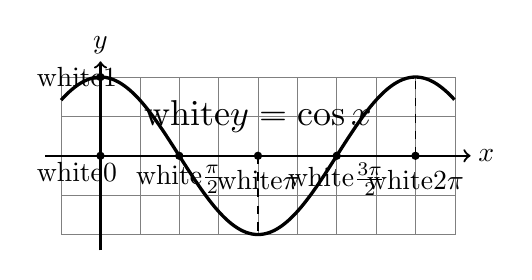
\begin{tikzpicture}

	% Grid
	\draw[step=0.5, very thin, gray] (-0.5,-1) grid ++(5, 2);

	% Graphs
	\draw[domain=-0.5:4.5,smooth,samples=500,variable=\x,black, very thick] plot ({\x},{cos(deg(\x/4*2*pi))});

	% Axes
	\draw[->, thick] (-0.7, 0) -- (4.7, 0);
	\draw[->, thick] (0, -1.2) -- (0, 1.2);

	\draw[-, dashed] (2, 0) -- (2, -1);
	\draw[-, dashed] (4, 0) -- (4, 1);

	% Nodes
	\draw (4.9,0) node {$x$};
	\draw (0, 1.4) node {$y$};

	\draw (-0.3, -0.2) node {\contour{white}{$0$}};
	\draw (-0.3, 1) node {\contour{white}{$1$}};

	\draw (1, -0.3) node {\contour{white}{$\frac{\pi}{2}$}};
	\draw (2, -0.3) node {\contour{white}{$\pi$}};
	\draw (3, -0.3) node {\contour{white}{$\frac{3\pi}{2}$}};
	\draw (4, -0.3) node {\contour{white}{$2\pi$}};

	\draw (2, 0.5) node[scale=1.3] {\contour{white}{$y=\cos x$}};

	% Points
	\fill [black] (0, 0) circle (1.5pt);
	\fill [black] (0, 1) circle (1.5pt);
	\fill [black] (1, 0) circle (1.5pt);
	\fill [black] (2, 0) circle (1.5pt);
	\fill [black] (3, 0) circle (1.5pt);
	\fill [black] (4, 0) circle (1.5pt);

\end{tikzpicture}
		&
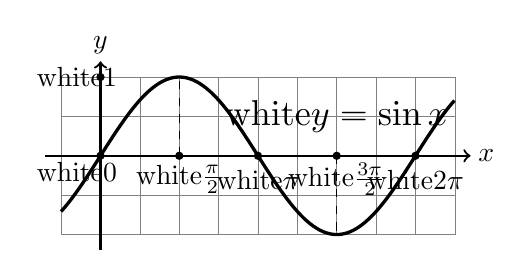
\begin{tikzpicture}

	% Grid
	\draw[step=0.5, very thin, gray] (-0.5,-1) grid ++(5, 2);

	% Graphs
	\draw[domain=-0.5:4.5,smooth,samples=500,variable=\x,black, very thick] plot ({\x},{sin(deg(\x/4*2*pi))});

	% Axes
	\draw[->, thick] (-0.7, 0) -- (4.7, 0);
	\draw[->, thick] (0, -1.2) -- (0, 1.2);

	\draw[-, dashed] (1, 0) -- (1, 1);
	\draw[-, dashed] (3, 0) -- (3, -1);

	% Nodes
	\draw (4.9,0) node {$x$};
	\draw (0, 1.4) node {$y$};

	\draw (-0.3, -0.2) node {\contour{white}{$0$}};
	\draw (-0.3, 1) node {\contour{white}{$1$}};

	\draw (1, -0.3) node {\contour{white}{$\frac{\pi}{2}$}};
	\draw (2, -0.3) node {\contour{white}{$\pi$}};
	\draw (3, -0.3) node {\contour{white}{$\frac{3\pi}{2}$}};
	\draw (4, -0.3) node {\contour{white}{$2\pi$}};

	\draw (3, 0.5) node[scale=1.3] {\contour{white}{$y=\sin x$}};

	% Points
	\fill [black] (0, 0) circle (1.5pt);
	\fill [black] (0, 1) circle (1.5pt);
	\fill [black] (1, 0) circle (1.5pt);
	\fill [black] (2, 0) circle (1.5pt);
	\fill [black] (3, 0) circle (1.5pt);
	\fill [black] (4, 0) circle (1.5pt);

\end{tikzpicture}
		\\
	\hline
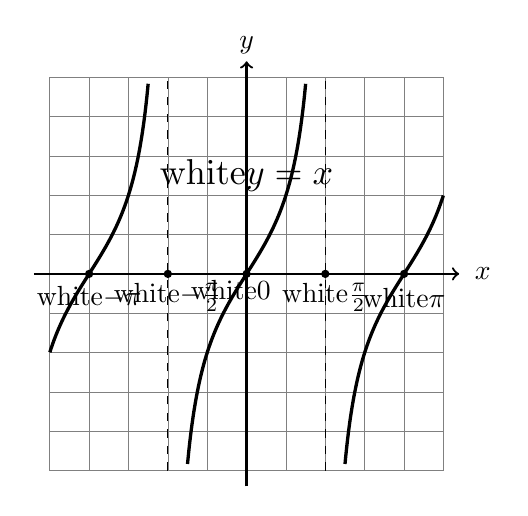
\begin{tikzpicture}

	% Grid
	\draw[step=0.5, very thin, gray] (-2.5,-2.5) grid ++(5, 5);

	% Graphs
	\draw[domain=-0.75:0.75	,smooth,samples=500,variable=\x,black, very thick] plot ({\x},{sin(deg(\x/4*2*pi))/cos(deg(\x/4*2*pi))});

	\draw[domain=1.25:2.5,smooth,samples=500,variable=\x,black, very thick] plot ({\x},{sin(deg(\x/4*2*pi))/cos(deg(\x/4*2*pi))});

	\draw[domain=-1.25:-2.5,smooth,samples=500,variable=\x,black, very thick] plot ({\x},{sin(deg(\x/4*2*pi))/cos(deg(\x/4*2*pi))});

	% Axes
	\draw[->, thick] (-2.7, 0) -- (2.7, 0);
	\draw[->, thick] (0, -2.7) -- (0, 2.7);

	\draw[-, dashed] (1, -2.5) -- (1, 2.5);
	\draw[-, dashed] (-1, -2.5) -- (-1, 2.5);

	% Nodes
	\draw (3,0) node {$x$};
	\draw (0, 2.9) node {$y$};

	\draw (-0.2, -0.2) node {\contour{white}{$0$}};

	\draw (1, -0.3) node {\contour{white}{$\frac{\pi}{2}$}};
	\draw (2, -0.3) node {\contour{white}{$\pi$}};
	\draw (-1, -0.3) node {\contour{white}{$-\frac{\pi}{2}$}};
	\draw (-2, -0.3) node {\contour{white}{$-\pi$}};

	\draw (0, 1.25) node[scale=1.3] {\contour{white}{$y=\tg x$}};

	% Points
	\fill [black] (0, 0) circle (1.5pt);
	\fill [black] (1, 0) circle (1.5pt);
	\fill [black] (2, 0) circle (1.5pt);
	\fill [black] (-1, 0) circle (1.5pt);
	\fill [black] (-2, 0) circle (1.5pt);

\end{tikzpicture}
		&
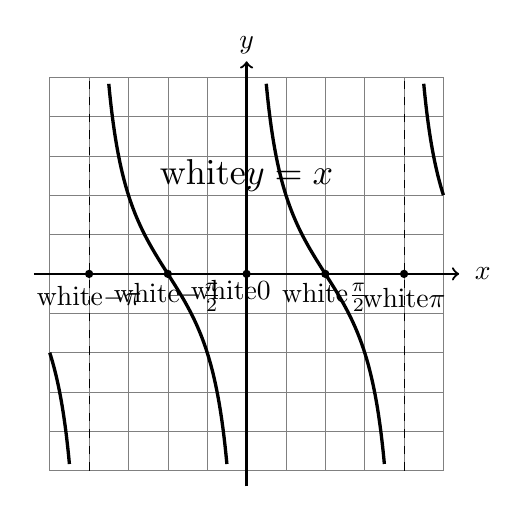
\begin{tikzpicture}

	% Grid
	\draw[step=0.5, very thin, gray] (-2.5,-2.5) grid ++(5, 5);

	% Graphs
	\draw[domain=0.25:1.75	,smooth,samples=500,variable=\x,black, very thick] plot ({\x},{cos(deg(\x/4*2*pi))/sin(deg(\x/4*2*pi))});

	\draw[domain=2.25:2.5,smooth,samples=500,variable=\x,black, very thick] plot ({\x},{cos(deg(\x/4*2*pi))/sin(deg(\x/4*2*pi))});

	\draw[domain=-0.25:-1.75,smooth,samples=500,variable=\x,black, very thick] plot ({\x},{cos(deg(\x/4*2*pi))/sin(deg(\x/4*2*pi))});

	\draw[domain=-2.25:-2.5,smooth,samples=500,variable=\x,black, very thick] plot ({\x},{cos(deg(\x/4*2*pi))/sin(deg(\x/4*2*pi))});

	% Axes
	\draw[->, thick] (-2.7, 0) -- (2.7, 0);
	\draw[->, thick] (0, -2.7) -- (0, 2.7);

	\draw[-, dashed] (2, -2.5) -- (2, 2.5);
	\draw[-, dashed] (-2, -2.5) -- (-2, 2.5);

	% Nodes
	\draw (3,0) node {$x$};
	\draw (0, 2.9) node {$y$};

	\draw (-0.2, -0.2) node {\contour{white}{$0$}};

	\draw (1, -0.3) node {\contour{white}{$\frac{\pi}{2}$}};
	\draw (2, -0.3) node {\contour{white}{$\pi$}};
	\draw (-1, -0.3) node {\contour{white}{$-\frac{\pi}{2}$}};
	\draw (-2, -0.3) node {\contour{white}{$-\pi$}};

	\draw (0, 1.25) node[scale=1.3] {\contour{white}{$y=\ctg x$}};

	% Points
	\fill [black] (0, 0) circle (1.5pt);
	\fill [black] (1, 0) circle (1.5pt);
	\fill [black] (2, 0) circle (1.5pt);
	\fill [black] (-1, 0) circle (1.5pt);
	\fill [black] (-2, 0) circle (1.5pt);

\end{tikzpicture}
		\\
	\hline
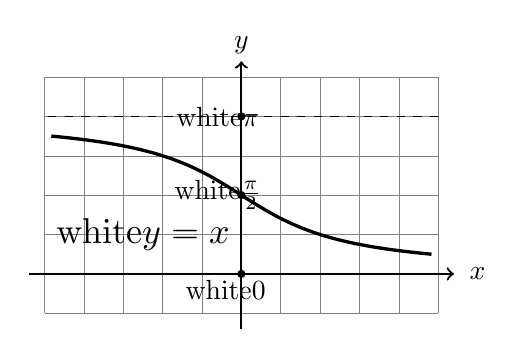
\begin{tikzpicture}

	% Grid
	\draw[step=0.5, very thin, gray] (-2.5,-0.5) grid ++(5, 3);

	% Graphs
	\draw[domain=0.25:1.75	,smooth,samples=500,variable=\x,black, very thick] plot ({cos(deg(\x/4*2*pi))/sin(deg(\x/4*2*pi))}, {\x});

	% Axes
	\draw[->, thick] (-2.7, 0) -- (2.7, 0);
	\draw[->, thick] (0, -0.7) -- (0, 2.7);

	\draw[-, dashed] (2.5, 2) -- (-2.5, 2);

	% Nodes
	\draw (3,0) node {$x$};
	\draw (0, 2.9) node {$y$};

	\draw (-0.2, -0.2) node {\contour{white}{$0$}};

	\draw (-0.3, 1) node {\contour{white}{$\frac{\pi}{2}$}};
	\draw (-0.3, 2) node {\contour{white}{$\pi$}};

	\draw (-1.25, 0.5) node[scale=1.3] {\contour{white}{$y=\arcctg x$}};

	% Points
	\fill [black] (0, 0) circle (1.5pt);
	\fill [black] (0, 1) circle (1.5pt);
	\fill [black] (0, 2) circle (1.5pt);

\end{tikzpicture}	
		&
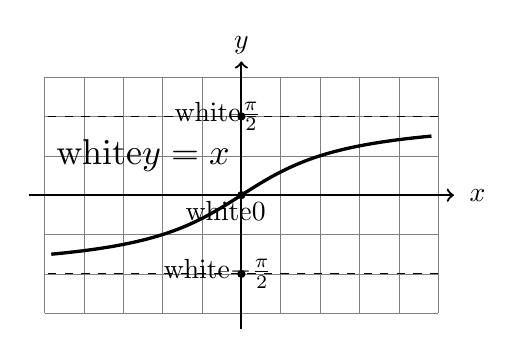
\begin{tikzpicture}

	% Grid
	\draw[step=0.5, very thin, gray] (-2.5,-1.5) grid ++(5, 3);

	% Graphs
	\draw[domain=-0.75:0.75	,smooth,samples=500,variable=\x,black, very thick] plot ({sin(deg(\x/4*2*pi))/cos(deg(\x/4*2*pi))}, {\x});

	% Axes
	\draw[->, thick] (-2.7, 0) -- (2.7, 0);
	\draw[->, thick] (0, -1.7) -- (0, 1.7);

	\draw[-, dashed] (2.5, 1) -- (-2.5, 1);
	\draw[-, dashed] (2.5, -1) -- (-2.5, -1);

	% Nodes
	\draw (3,0) node {$x$};
	\draw (0, 1.9) node {$y$};

	\draw (-0.2, -0.2) node {\contour{white}{$0$}};

	\draw (-0.3, 1) node {\contour{white}{$\frac{\pi}{2}$}};
	\draw (-0.3, -1) node {\contour{white}{$-\frac{\pi}{2}$}};

	\draw (-1.25, 0.5) node[scale=1.3] {\contour{white}{$y=\arctg x$}};

	% Points
	\fill [black] (0, 0) circle (1.5pt);
	\fill [black] (0, 1) circle (1.5pt);
	\fill [black] (0, -1) circle (1.5pt);

\end{tikzpicture}
		\\
	\hline
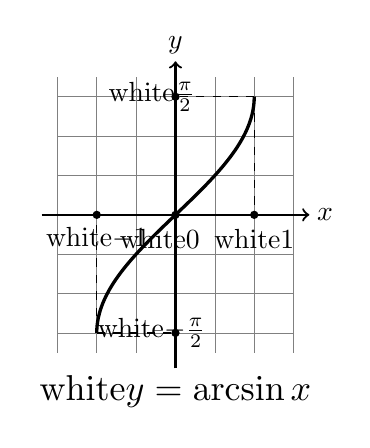
\begin{tikzpicture}

	% Grid
	\draw[step=0.5, very thin, gray] (-1.5,-1.75) grid ++(3, 3.5);

	% Graphs
	\draw[domain=-1.5:1.5, smooth,samples=500,variable=\x,black, very thick] plot ({sin(deg(\x/3*pi))}, {\x});

	% Axes
	\draw[->, thick] (-1.7, 0) -- (1.7, 0);
	\draw[->, thick] (0, -1.95) -- (0, 1.95);

	\draw[-, dashed] (-1, -1.5) -- (-1, 0);
	\draw[-, dashed] (1, 1.5) -- (1, 0);

	\draw[-, dashed] (-1, -1.5) -- (0, -1.5);
	\draw[-, dashed] (1, 1.5) -- (0, 1.5);

	% Nodes
	\draw (1.9,0) node {$x$};
	\draw (0, 2.15) node {$y$};

	\draw (-0.2, -0.3) node {\contour{white}{$0$}};

	\draw (-0.3, 1.5) node {\contour{white}{$\frac{\pi}{2}$}};
	\draw (-0.3, -1.5) node {\contour{white}{$-\frac{\pi}{2}$}};
	\draw (-1, -0.3) node {\contour{white}{$-1$}};
	\draw (1, -0.3) node {\contour{white}{$1$}};

	\draw (0, -2.25) node[scale=1.3] {\contour{white}{$y=\arcsin x$}};

	% Points
	\fill [black] (0, 0) circle (1.5pt);
	\fill [black] (0, 1.5) circle (1.5pt);
	\fill [black] (0, -1.5) circle (1.5pt);
	\fill [black] (1, 0) circle (1.5pt);
	\fill [black] (-1, 0) circle (1.5pt);

\end{tikzpicture}	
		&
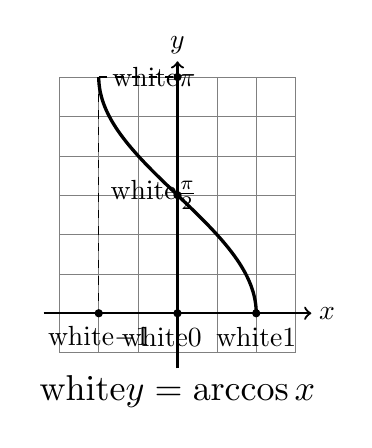
\begin{tikzpicture}

	% Grid
	\draw[step=0.5, very thin, gray] (-1.5,-0.5) grid ++(3, 3.5);

	% Graphs
	\draw[domain=0:3, smooth,samples=500,variable=\x,black, very thick] plot ({cos(deg(\x/3*pi))}, {\x});

	% Axes
	\draw[->, thick] (-1.7, 0) -- (1.7, 0);
	\draw[->, thick] (0, -0.7) -- (0, 3.2);

	\draw[-, dashed] (-1, 3) -- (-1, 0);
	\draw[-, dashed] (-1, 3) -- (0, 3);

	% Nodes
	\draw (1.9,0) node {$x$};
	\draw (0, 3.4) node {$y$};

	\draw (-0.2, -0.3) node {\contour{white}{$0$}};

	\draw (-0.3, 1.5) node {\contour{white}{$\frac{\pi}{2}$}};
	\draw (-0.3, 3) node {\contour{white}{$\pi$}};
	\draw (-1, -0.3) node {\contour{white}{$-1$}};
	\draw (1, -0.3) node {\contour{white}{$1$}};

	\draw (0, -1) node[scale=1.3] {\contour{white}{$y=\arccos x$}};

	% Points
	\fill [black] (0, 0) circle (1.5pt);
	\fill [black] (0, 1.5) circle (1.5pt);
	\fill [black] (0, 3) circle (1.5pt);
	\fill [black] (1, 0) circle (1.5pt);
	\fill [black] (-1, 0) circle (1.5pt);

\end{tikzpicture}
		\\
	\hline
\end{tabu}

\begin{tabu}[t]{||c|c||}
	\hline
		\multicolumn{2}{||c||}{\textbf{Основное}} \\
	\hline
	\hline
		$\displaystyle \sin^2 \alpha + \cos^2 \alpha = 1 $ &
		$\displaystyle \sin \alpha = \cos \left(\frac{\pi}{2}-\alpha\right) $ \\
	\hline
		$\displaystyle \tg^2 \alpha + 1 = \frac{1}{\cos^2 \alpha} $ &
		$\displaystyle \ctg^2 \alpha + 1 = \frac{1}{\sin^2 \alpha} $ \\
	\hline
		$\displaystyle \tg \alpha\, \ctg \alpha = 1 $ &
		$\displaystyle \tg \alpha = \frac{\sin \alpha}{\cos \alpha} $ \\
	\hline
\end{tabu}

\begin{tabu}[t]{||c||}
	\hline
		\textbf{Суммы углов} \\
	\hline
	\hline
		$\displaystyle \sin(\alpha\pm \beta) = \sin \alpha\, \cos \beta \pm \cos \alpha\, \sin \beta $ \\
	\hline
		$\displaystyle \cos(\alpha\pm \beta) = \cos \alpha\, \cos \beta \mp \sin \alpha\, \sin \beta $ \\
	\hline
		$\displaystyle \tg (\alpha \pm \beta) = \frac{\tg \alpha \pm \tg \beta}{1 \mp \tg \alpha \, \tg \beta} $ \\
	\hline
\end{tabu}

\begin{tabu}[t]{||c||}
	\hline
		\textbf{Двойные и тройные углы} \\
	\hline
	\hline
		$ \sin 2\, \alpha = 2\, \sin \alpha\, \cos \alpha $ \\
	\hline
		\specialcell{$\displaystyle \cos 2\, \alpha = \cos^2 \alpha - \sin^2 \alpha = $ \\ $\displaystyle 2\, \cos^2 \alpha - 1 = 1 - 2\, \sin^2 \alpha $} \\
	\hline
		$\displaystyle \tg 2\alpha = \frac{2\, \tg \alpha}{1 - \tg^2 \alpha} = \frac{2}{\ctg \alpha - \tg \alpha} $ \\
	\hline
		$\displaystyle \cos 3\, \alpha = 4\, \cos^3 \alpha - 3\, \cos \alpha $ \\
	\hline
		$\displaystyle \sin 3\, \alpha = 3\, \sin \alpha - 4\, \sin^3 \alpha $ \\
	\hline
		$\displaystyle \tg 3\, \alpha = \frac{3\, \tg \alpha - \tg^3 \alpha}{1 - 3\, \tg^2 \alpha} $ \\
	\hline
\end{tabu}

\begin{tabu}[t]{||c||}
	\hline
		\textbf{Сумма функций} \\
	\hline
	\hline
		$\displaystyle \sin \alpha \pm \sin \beta = 2\, \sin \frac{\alpha \pm \beta}{2}\, \cos \frac{\alpha \mp \beta}{2} $ \\
	\hline
		$\displaystyle \cos \alpha \pm \cos \beta = 2\, \cos \frac{\alpha \pm \beta}{2}\, \cos \frac{\alpha \mp \beta}{2} $ \\
	\hline
		$\displaystyle \tg \alpha \pm \tg \beta = \frac{\sin (\alpha \pm \beta)}{\cos \alpha\, \cos \beta} $ \\
	\hline
		$\displaystyle \ctg \alpha \pm \ctg \beta = \frac{\pm\sin (\alpha \pm \beta)}{\sin \alpha\, \sin \beta} $ \\
	\hline
		$\displaystyle \ctg \alpha \pm \tg \beta = \frac{\cos (\alpha \mp \beta)}{\sin \alpha\, \cos \beta} $ \\
	\hline
		\specialcell{$\displaystyle a\, \sin \alpha + b\, \cos \alpha = $ \\ $\displaystyle = \sqrt{\mathstrut a^2 + b^2}\, \sin \left(\alpha + \arcsin \frac{a}{\sqrt{\mathstrut a^2 + b^2}}\right) $} \\
	\hline
		\specialcell{$\displaystyle \sin x \pm \cos x = \pm\sqrt{2} \sin\left(x \pm \frac{\pi}{4}\right) = $ \\ $\displaystyle = \pm\sqrt{2} \cos\left(x \mp \frac{\pi}{4}\right) $} \\
	\hline
\end{tabu}

\begin{tabu}[t]{||c||}
	\hline
		\textbf{Произведение функций} \\
	\hline
	\hline
		$\displaystyle \sin \alpha\, \cos \beta = \frac{1}{2}\, (\sin (\alpha - \beta) + \sin (\alpha + \beta)) $ \\
	\hline
		$\displaystyle \sin \alpha\, \sin \beta = \frac{1}{2}\, (\cos (\alpha - \beta) - \cos (\alpha + \beta)) $ \\
	\hline
		$\displaystyle \cos \alpha\, \cos \beta = \frac{1}{2}\, (\cos (\alpha - \beta) + \cos (\alpha + \beta)) $ \\
	\hline
\end{tabu}

\begin{tabu}[t]{||c|c||}
	\hline
		\multicolumn{2}{||c||}{\textbf{Понижение степени и половинный угол}} \\
	\hline
	\hline
		$\displaystyle \cos^2 \alpha = \frac{1 + \cos 2\, \alpha}{2} $ &
		$\displaystyle \sin^2 \alpha = \frac{1 - \cos 2\, \alpha}{2} $ \\
	\hline
		\multicolumn{2}{||c||}{$\displaystyle \sin^3 \alpha = \frac14(3\sin \alpha - \sin 3 \alpha) $} \\		
	\hline
		\multicolumn{2}{||c||}{$\displaystyle \cos^3 \alpha = \frac14(3\cos \alpha + \cos 3 \alpha) $} \\
	\hline
		\multicolumn{2}{||c||}{$\displaystyle \tg \frac{\alpha}{2} = \pm \sqrt{\mathstrut \frac{1 - \cos \alpha}{1 + \cos \alpha}} = \frac{\sin \alpha}{1 + \cos \alpha} = \frac{1-\cos \alpha}{\sin \alpha} $} \\
	\hline
\end{tabu}

\begin{tabu}[t]{||c|c|c|c|c|c|c|c|c||}
	\hline
		\multicolumn{9}{||c||}{\textbf{Формулы приведения}} \\
	\hline
	\hline
		$ \alpha $ &
			\specialcell{$ \frac{\pi}{2} - \alpha $ \\ $ 90^{\circ} - \alpha $} &
			\specialcell{$ \frac{\pi}{2} + \alpha $ \\ $ 90^{\circ} + \alpha $} &
			\specialcell{$ \pi - \alpha $ \\ $ 180^{\circ} - \alpha $} &
			\specialcell{$ \pi + \alpha $ \\ $ 180^{\circ} + \alpha $} &
			\specialcell{$ \frac{3\, \pi}{2} - \alpha $ \\ $ 270^{\circ} - \alpha $} &
			\specialcell{$ \frac{3\, \pi}{2} + \alpha $ \\ $ 270^{\circ} + \alpha $} &
			\specialcell{$ 2\, \pi - \alpha $ \\ $ 360^{\circ} - \alpha $} &
			\specialcell{$ 2\, \pi + \alpha $ \\ $ 360^{\circ} + \alpha $} \\
	\hline
		$ \sin \alpha $ & 	$ \cos \alpha $ & 	$ \cos \alpha $ & 	$ \sin \alpha $ & 	$ -\sin \alpha $ & 	$ -\cos \alpha $ & 	$ -\cos \alpha $ & 	$ -\sin \alpha $ & 	$ \sin \alpha $ \\
	\hline
		$ \cos \alpha $ & 	$ \sin \alpha $ & 	$ -\sin \alpha $ & 	$ -\cos \alpha $ & 	$ -\cos \alpha $ & 	$ -\sin \alpha $ & 	$ \sin \alpha $ & 	$ \cos \alpha $ & 	$ \cos \alpha $ \\
	\hline
		$ \tg \alpha $ & 	$ \ctg \alpha $ & 	$ -\ctg \alpha $ & 	$ -\tg \alpha $ & 	$ \tg \alpha $ & 	$ \ctg \alpha $ & 	$ -\ctg \alpha $ & 	$ -\tg \alpha $ & 	$ \tg \alpha $ \\
	\hline
		$ \ctg \alpha $ & 	$ \tg \alpha $ & 	$ -\tg \alpha $ & 	$ -\ctg \alpha $ & 	$ \ctg \alpha $ & 	$ \tg \alpha $ & 	$ -\tg \alpha $ & 	$ -\ctg \alpha $ & 	$ \ctg \alpha $ \\
	\hline
\end{tabu}

\begin{tabu}[t]{||c|c|c||}
	\hline
		\multicolumn{3}{||c||}{\textbf{Тригонометрические уравнения}} \\
	\hline
	\hline
		Уравнение & Решение & Условие \\
	\hline
		$ \sin x = a $ & 	$ x = (-1)^k\, \arcsin a + \pi\, k $ & 	$ |a| \le 1 $ \\
	\hline
		$ \cos x = a $ & 	$ x = \pm \arccos a + 2\, \pi\, k $ & 	$ |a| \le 1 $ \\
	\hline
		$ \tg x = a $ & 	$ x = \arctg a + \pi\, k $ & 	$ - $ \\
	\hline
		$ \ctg x = a $ & 	$ x = \arcctg a + \pi\, k $ & 	$ - $ \\
	\hline
\end{tabu}

\begin{tabu}[t]{||c|c||c|c||}
	\hline
		\multicolumn{4}{||c||}{\textbf{Частные случаи тригонометрических уравнений}} \\
	\hline
	\hline
		Уравнение & Решение & Уравнение & Решение \\
	\hline
		$ \sin x = 0 $ & 	$ x = \pi\, k $ & 				$ \cos x = 0 $ &	$ x = \frac{\pi}{2} + \pi\, k $ \\
	\hline
		$ \sin x = 1 $ & 	$ x = \frac{\pi}{2} + 2\, \pi\, k $ & 	$ \cos x = 1 $ & 	$ x = 2\, \pi\, k $ \\
	\hline
		$ \sin x = -1 $ & 	$ x = -\frac{\pi}{2} + 2\, \pi\, k $ & 	$ \cos x = -1 $ & 	$ x = \pi + 2\, \pi\, k $ \\
	\hline
		$ \tg x = 0 $ & 	$ x = \pi\, k $ & 				$ \ctg x = 0 $ & 	$ x = \frac{\pi}{2} + \pi\, k $ \\
	\hline
		$ \tg x = 1 $ & 	$ x = \frac{\pi}{4} + \pi\, k $ & 		$ \ctg x = 1 $ & 	$ x = \frac{\pi}{4} + \pi\, k $ \\
	\hline
		$ \tg x = -1 $ & 	$ x = -\frac{\pi}{4} + \pi\, k $ & 		$ \ctg x = -1 $ & 	$ x = \frac{3\, \pi}{4} + \pi\, k $ \\
	\hline
\end{tabu}

\begin{tabu}[t]{||c||c||c||}
	\hline
		\multicolumn{3}{||c||}{\textbf{Обратные тригонометрические функции}} \\
	\hline
	\hline
		$ \sin\arcsin x = x $            & $ \sin\arccos x = \sqrt{1-x^2} $          & $ \arcsin(-x) = -\arcsin x $              \\
	\hline
		$ \arcsin\sin\alpha = \alpha $   & $ \cos\arcsin x = \sqrt{1-x^2} $            & $ \arccos(-x) = \pi - \arccos x $         \\
	\hline
	\hline
		$ \cos\arccos x = x $            & $ \sin\arctg x = \frac{x}{\sqrt{1+x^2}} $ & $ \arctg(-x) = -\arctg x $                \\
	\hline
		$ \arccos\cos\alpha = \alpha $   & $ \cos\arctg x = \frac{1}{\sqrt{1+x^2}} $ & $ \arcctg(-x) = \pi - \arcctg x $         \\
	\hline
	\hline
		$ \tg\arctg x = x $              & $ \tg\arcsin x = \frac{x}{\sqrt{1-x^2}} $ & $ \arcsin x + \arccos x = \frac{\pi}{2} $ \\
	\hline
		$ \arctg\tg\alpha = \alpha $     & $ \tg\arccos x = \frac{\sqrt{1-x^2}}{x} $ & $ \arctg x + \arcctg x = \frac{\pi}{2} $  \\
	\hline
\end{tabu}

\begin{tabu}[t]{||c||}
	\hline
		\textbf{Сумма обратных триг. функций} \\
	\hline
	\hline
		$ \arcsin x - \arcsin y =  \arcsin x + \arcsin(-y) $ \\
		$ \Sigma_{\sin{}} = \arcsin\left(x\sqrt{\mathstrut 1-y^2}+y\sqrt{\mathstrut 1-x^2}\right) $ \\
	\hline
		$ \boxed{\arcsin x + \arcsin y =} $ \\
		$ \left\{ \begin{aligned}
			\Sigma_{\sin{}}, \quad & xy \leqslant 0,\quad & x^2 + y^2 \leqslant 1 \\
			\pi-\Sigma_{\sin{}}, \quad & x > 0, y > 0,\quad  & x^2 + y^2 > 1 \\
			-\pi-\Sigma_{\sin{}}, \quad & x < 0, y < 0,\quad & x^2 + y^2 > 1 \\
		\end{aligned} \right. $ \\
	\hline
	\hline
		$ \arccos x - \arccos y =  -\pi + \arccos x + \arccos(-y) $ \\
		$ \Sigma_{\cos{}} = \arccos\left(xy+\sqrt{\mathstrut 1-x^2}\sqrt{\mathstrut 1-y^2}\right) $ \\
	\hline
		$ \boxed{\arccos x + \arccos y =} $
		$ \left\{ \begin{aligned}
			\Sigma_{\cos{}}, \quad & x \geqslant -y \\
			2\pi-\Sigma_{\cos{}}, \quad & x < -y
		\end{aligned} \right. $ \\
	\hline
	\hline
		$ \arctg x - \arctg y =  \arctg x + \arctg(-y) $ \\
		$ \Sigma_{\tg{}} = \arctg\frac{x+y}{1-xy} $ \\
	\hline
		$ \boxed{\arctg x + \arctg y =} $
		$ \left\{ \begin{aligned}
			\Sigma_{\tg{}}, \quad & & xy < 1 \\
			\pi+\Sigma_{\tg{}}, \quad & x > 0, \quad & xy>1 \\
			-\pi+\Sigma_{\tg{}}, \quad & x < 0, \quad & xy>1 \\
		\end{aligned} \right. $ \\
	\hline
\end{tabu}

\begin{tabu}[t]{||c|c|c|c|c|c|c|c|c|c||}
	\hline
		\multicolumn{10}{||c||}{\textbf{Таблица значений для стандартных углов}} \\
	\hline
	\hline
		$ \alpha $ &
		$ 0 $ &
		$ \cfrac{\pi}{6} $ &
		$ \cfrac{\pi}{4} $ &
		$ \cfrac{\pi}{3} $ &
		$ \cfrac{\pi}{2} $ &
		$ \cfrac{2\pi}{3} $ &
		$ \cfrac{3\pi}{4} $ &
		$ \cfrac{5\pi}{6} $ &
		$ \pi $ \\
	\hline
		$ \alpha^{\circ} $ &
		$ 0^{\circ} $ &
		$ 30^{\circ} $ &
		$ 45^{\circ} $ &
		$ 60^{\circ} $ &
		$ 90^{\circ} $ &
		$ 120^{\circ} $ &
		$ 135^{\circ} $ &
		$ 150^{\circ} $ & 
		$ 180^{\circ} $ \\
	\hline
		$ \sin \alpha $ & 	$ 0 $ & 	$ \cfrac{1}{2} $ & 	$ \cfrac{\sqrt{2}}{2} $ & 	$ \cfrac{\sqrt{3}}{2} $ & 	$ 1 $ & 	$ \cfrac{\sqrt{3}}{2} $ & 	$ \cfrac{\sqrt{2}}{2} $ & 	$ \cfrac{1}{2} $ & $ 0 $ \\
	\hline
		$ \cos \alpha $ & 	$ 1 $ & 	$ \cfrac{\sqrt{3}}{2} $ & 	$ \cfrac{\sqrt{2}}{2} $ & 	$ \cfrac{1}{2} $ & 	$ 0 $ & 	$ -\cfrac{1}{2} $ & 	$ -\cfrac{\sqrt{2}}{2} $ & 	$ -\cfrac{\sqrt{3}}{2} $ & $ -1 $ \\
	\hline
		$ \tg \alpha $ & 	$ 0 $ & 	$ \cfrac{\sqrt{3}}{3} $ & 	$ 1 $ & 	$ \sqrt{3} $ & 	--- & 	$ -\sqrt{3} $ & 	$ -1 $ & 	$ -\cfrac{\sqrt{3}}{3} $ & $ 0 $ \\
	\hline
		$ \ctg \alpha $ & 	--- & 	$ \sqrt{3} $ & 	$ 1 $ & 	$ \cfrac{\sqrt{3}}{3} $ & 	0 & 	$ -\cfrac{\sqrt{3}}{3} $ & 	$ -1 $ & 	$ -\sqrt{3} $ & --- \\
	\hline
\end{tabu}

\begin{tabu}[t]{||c|c|c|c|c|c|c||}
	\hline
		\multicolumn{7}{||c||}{\textbf{Таблица значений для особых углов}} \\
	\hline
	\hline
		$ \alpha $ &
			$ \cfrac{\pi}{12}  =  15^{\circ} $ &
			$ \cfrac{\pi}{10} = 18^{\circ} $ &
			$ \cfrac{\pi}{5} = 36^{\circ} $ &
			$ \cfrac{3\pi}{10} = 54^{\circ} $ &
			$ \cfrac{2\pi}{5} = 72^{\circ} $ &
			$ \cfrac{5\pi}{12} = 75^{\circ} $ \\
	\hline
		$ \sin \alpha $ &
		$ \cfrac{\sqrt{3}-1}{2\sqrt{2}} $ & 	
		$ \cfrac{\sqrt{5}-1}{4} $ & 	
		$ \cfrac{\sqrt{5-\sqrt{5}}}{2\sqrt{2}} $ & 	
		$ \cfrac{\sqrt{5}+1}{4} $ & 	
		$ \cfrac{\sqrt{5+\sqrt{5}}}{2\sqrt{2}} $ & 	
		$ \cfrac{\sqrt{3}+1}{2\sqrt{2}} $ \\
	\hline
		$ \cos \alpha $ & 	
		$ \cfrac{\sqrt{3}+1}{2\sqrt{2}} $ & 	
		$ \cfrac{\sqrt{5+\sqrt{5}}}{2\sqrt{2}} $ & 	
		$ \cfrac{\sqrt{5}+1}{4} $ & 	
		$ \cfrac{\sqrt{5-\sqrt{5}}}{2\sqrt{2}} $ & 	
		$ \cfrac{\sqrt{5}-1}{4} $ & 	
		$ \cfrac{\sqrt{3}-1}{2\sqrt{2}} $ \\
	\hline
		$ \tg \alpha $ & 	
		$ 2-\sqrt{3} $ & 	
		$ \sqrt{1-\cfrac{2}{\sqrt{5}}} $ & 	
		$ \sqrt{5-2\sqrt{5}} $ & 	
		$ \sqrt{1+\cfrac{2}{\sqrt{5}}} $ & 	
		$ \sqrt{5+2\sqrt{5}} $ & 	
		$ 2+\sqrt{3} $ \\
	\hline
		$ \ctg \alpha $ & 
		$ 2+\sqrt{3} $ & 	
		$ \sqrt{5+2\sqrt{5}} $ & 	
		$ \sqrt{1+\cfrac{2}{\sqrt{5}}} $ & 	
		$ \sqrt{5-2\sqrt{5}} $ & 	
		$ \sqrt{1-\cfrac{2}{\sqrt{5}}} $ & 	
		$ 2-\sqrt{3} $ \\
	\hline
\end{tabu}

%--------------------------------------------------------------------------------%

\section{Гиперболические функции}

\subsection{Графики}

\subsection{Основные}

$ \ch^2 x - \sh^2 x = 1 $

$ \ctg^2 x - 1 = \frac{1}{\sh^2 x} $

$ 1 - \th^2 x = \frac{1}{\ch^2 x} $

$ \th x \, \cth x = 1 $

$ \th x = \frac{\sh x}{\ch x} $

\subsection{Суммы углов}

$ \sh(x \pm y) = \sh x \, \ch y \pm \sh y \, \ch x $

$ \ch(x \pm y) = \ch x \, \ch y \pm \sh y \, \sh x $

$ \th(x \pm y) = \frac{\th x \pm \th y}{1 \pm \th x \, \th y} $

\subsection{Двойные и тройные углы}

$ \sh 2x = 2\sh x \, \ch x $

$ \ch 2x = \ch^2 x + \sh^2 x = 2\ch^2 x - 1 = 1 + 2\sh^2 x $

$ \th 2x = \frac{2\th x}{1 + \th^2 x} = \frac{2}{\th x + \cth x} $

$ \sh 3x = 4\sh^3 x + 3\sh x $

$ \ch 3x = 4\ch^3 x - 3\ch x $

$ \th 3x = \th x \cdot \frac{3+\th^2 x}{1 + 3\th^2 x} $

\subsection{Сумма функций}

$ \sh x \pm \sh y = 2\sh\frac{x\pm y}{2}\,\ch\frac{x\mp y}{2} $

$ \ch x + \ch y = 2\ch\frac{x+y}{2}\,\ch\frac{x-y}{2} $

$ \ch x - \ch y = 2\sh\frac{x+ y}{2}\,\sh\frac{x- y}{2} $

$ \th x \pm \th y = 2\frac{\sh(x\pm y)}{\ch x\, \ch y} $

\subsection{Произведение функций}

$ \sh x \, \sh y = \frac12(\ch(x+y)-\ch(x-y)) $

$ \sh x \, \ch y = \frac12(\sh(x+y)+\sh(x-y)) $

$ \ch x \, \ch y = \frac12(\ch(x+y)+\ch(x-y)) $

\subsection{Понижение степени и половинный угол}

$ \ch^2 x = \frac{\ch 2x+1}{2} $

$ \th^2 x = \frac{\ch 2x-1}{2} $ 

\subsection{Универсальная гиперболическая подстановка}



\subsection{Обратные гиперболические функции}

%--------------------------------------------------------------------------------%

\section{Математический анализ}

\subsection{Пределы}

\begin{tabu}[t]{||l|l|l|l||}
	\hline
		\multicolumn{4}{||c||}{\textbf{Различия между \boldmath$\inf$ и \boldmath$\max$; \boldmath$\sup$ и \boldmath$\min$:}} \\
	\hline
	\hline
		$ \sup[0, 2] = 0 $ & $ \sup(0, 2] = 0$ & $ \sup[0, 2) = 0 $ & $\sup(0, 2) = 0 $ \\
	\hline
		$ \min[0, 2] = 0 $ & $ \min(0, 2] \nexists$ & $ \min[0, 2) = 0 $ & $\min(0, 2) \nexists $ \\
	\hline
		$ \inf[0, 2] = 2 $ & $ \inf(0, 2] = 2$ & $ \inf[0, 2) = 2 $ & $\inf(0, 2) = 2 $ \\
	\hline
		$ \max[0, 2] = 2 $ & $ \max(0, 2] = 2$ & $ \max[0, 2) \nexists $ & $\max(0, 2) \nexists $ \\
	\hline
\end{tabu}

\subsubsection{Арифметика пределов}

$\displaystyle \lim_{n\to \infty} a_n = A, \lim_{n\to \infty} b_n = B $

1. $\displaystyle \lim_{n\to \infty} c\cdot a_n = c\cdot A, c \in \mathbb{R}, \text{if} A = \infty \text{then} c \neq 0  $

2. $\displaystyle \lim_{n\to \infty} (a_n \pm b_n) = A\pm B, A\neq\infty, B\neq\infty $

3. $\displaystyle \lim_{n\to \infty} (a_n\cdot b_n) = A\cdot B, A\cdot B \neq 0\cdot\infty $

4. $\displaystyle \lim_{n\to \infty} \frac{a_n}{b_n} = \frac{A}{B}, B\neq 0, \frac{A}{B} \neq \frac{\infty}{\infty}, \frac{A}{B} \neq \frac{0}{0} $

\subsubsection{Замечательные и элементарные пределы:}

$\displaystyle \lim_{n\to \infty} q^n = \left\{ \begin{aligned}
		&\infty, &&q > 1 \\
		&0, &&0 < q < 1 \\
		&1, &&q = 1
	\end{aligned} \right. $

$\displaystyle \lim_{n\to \infty} \sqrt[n]{a} = 1 $

$\displaystyle \lim_{n\to \infty} \sqrt[n]{n} = 1 $

$\displaystyle \lim_{n\to \infty} \left( 1 + \frac{1}{n} \right)^n = e $

$\displaystyle \lim_{n\to \infty} \frac{e^x - 1}{x} = 1 $

$\displaystyle \lim_{n\to \infty} \frac{a^x - 1}{x} = \ln a $

$\displaystyle \lim_{n\to \infty} \frac{\ln(1+x)}{x} = 1 $

$\displaystyle \lim_{n\to \infty} \frac{\sin x}{x} = 1 $

$\displaystyle \lim_{n\to \infty} \frac{\tg x}{x} = 1 $

$\displaystyle \lim_{n\to \infty} \frac{1 - \cos x}{x^2} = \frac12 $

$\displaystyle \lim_{n\to \infty} \frac{\arcsin x}{x} = 1 $

$\displaystyle \lim_{n\to \infty} \frac{\arctg x}{x} = 1 $

\subsubsection{Теорема Лопиталя:}

Если

1. $\displaystyle \lim_{n\to \infty} f(x) = \lim_{n\to \infty} g(x) = 0 \text{ или } \infty $

2. $\displaystyle f $ и $\displaystyle g $ - дифференцируемые в $\displaystyle U_\varepsilon(x_0) $

то

$\displaystyle \lim_{n\to \infty} \frac{f(x)}{g(x)} = \lim_{n\to \infty} \frac{f'(x)}{g'(x)} $

\subsubsection{Эквивалентности:}

Таблица эквивалетностей при $\displaystyle x\to 0 $.

$\displaystyle \begin{aligned}
	\sin x & \sim & x \\
	\tg x & \sim & x \\
	\cos x & \sim & 1 - \frac{x^2}{2} \\
	\arcsin x & \sim & x \\
	\arctg x & \sim & x \\
	e^x & \sim & 1 + x \\
	a^x & \sim & 1 + x\ln a \\
	\ln (1 + x) & \sim & x \\
	(1+x)^\alpha & \sim & 1 + \alpha x \\
	\begin{aligned}
		a_0 x^n + a_1 x^{n-1} + \\
		+ \ldots + a_n
	\end{aligned} & \sim & a_0 x^n \\
	n! & \sim & \left(\frac{n}{e}\right)^n 
\end{aligned} $

\subsubsection{Шкала роста:}

При $\displaystyle n\to\infty $

$\displaystyle \ln^a n < n^b < \alpha^n < n! < n^n $

$\displaystyle a > 0, b > 0, \alpha > 1 $

\subsection{Дифференциирование}

\subsubsection{Свойства}

Арифметика производных:

$ (f(x) + g(x))' = f'(x) + g'(x) $

$ (f(x)\cdot g(x))' = f'(x)\cdot g(x) + f(x)\cdot g'(x) $

$ (k\cdot f(x))' = k\cdot f'(x), k \in R $

$ \left(\frac{f(x)}{g(x)}\right)' = \frac{f'(x)\cdot g(x) - f(x)\cdot g'(x)}{g^2(x)} $

Производная сложной функции:

$ (h(f(x)))' = h'(f(x)) \cdot f'(x) $

Дифференцирование больших произведений:

$ y' = y\cdot(\ln y)' $

- далее $\ln y$ раскладывается в сумму, и от каждого слагаемого отдельно берется производная.

Связь дифференциалов и производных:

$ f'(x) = \frac{df(x)}{dx} $

$ df(x) = f'(x) dx $

Производная обратной функции:

$ y = f(x), \quad x = f^{-1}(y) $

$ (f(x))' = \frac{1}{(f^{-1}(y))'} $

Арифметика дифференциалов:

TODO НАПИСАТЬ

\begin{tabu}[t]{||c|c||c|c||}
	\hline
		\multicolumn{4}{||c||}{\textbf{Таблица производных}} \\
	\hline
	\hline
		$ f(x) $ & $ f'(x) $ & $ f(x) $ &  $ f'(x) $ \\
	\hline
		$ c $ & $ 0 $ & $ \tg x $ &  $ \frac{1}{\cos^2 x} $ \\
	\hline
		$ x^n $ & $ nx^{n-1} $ & $ \ctg x $ &  $ -\frac{1}{\sin^2 x} $ \\
	\hline
		$ \sqrt{x} $ & $ \frac{1}{2\sqrt{x}} $ & $ \arcsin x $ &  $ \frac{1}{\sqrt{1-x^2}} $ \\
	\hline
		$ \frac{1}{x} $ & $ -\frac{1}{x^2} $ & $ \arccos x $ &  $ -\frac{1}{\sqrt{1-x^2}} $ \\
	\hline
		$ a^x $ & $ a^x \ln a $ & $ \arctg x $ &  $ \frac{1}{1+x^2} $ \\
	\hline
		$ e^x $ & $ e^x $ & $ \arcctg x $ &  $ -\frac{1}{1+x^2} $ \\
	\hline
		$ \log_a x $ & $ \frac{1}{x \ln a} $ & $ \sqrt[n]{x} $ &  $ \frac{1}{n\sqrt[n]{x^n-1}} $ \\
	\hline
		$ \ln x $ & $ \frac{1}{x} $ & $ \frac{1}{x^n} $ &  $ -\frac{n}{x^{n+1}} $ \\
	\hline
		$ \sin x $ & $ \cos x $ & $ \frac{1}{\sqrt{x}} $ &  $ -\frac{1}{2x\sqrt{x}} $ \\
	\hline
		$ \cos x $ & $ -\sin x $ & $ (x^n)^{(k)} $ & $ \binom nk k! x^{n-k} $ \\
	\hline
		 $ \sin^{(k)}(x) $ & $ \sin\left(x + \frac{\pi k}{2}\right) $ & $ \cos^{(k)}(x) $ &  $ \cos\left(x + \frac{\pi k}{2}\right) $ \\
	\hline
\end{tabu}

\subsection{Ряды}

\subsubsection{Признаки сходимости рядов:}

\begin{tabu}[t]{||c||c||}
	\hline
		\multicolumn{1}{||p{6cm}||}{\raggedright 
			Ряд сходится(сх-ся), если сходится последовательность его частичных сумм.
		} & \multicolumn{1}{p{6cm}||}{\raggedright 
			Если $\displaystyle \sum_{n=1}^\infty a_n $ сх-ся, то $ \forall c \in \mathbb{R} \Rightarrow \sum_{n=1}^\infty c\cdot a_n $ - сх-ся.
		} \\
	\hline
		\multicolumn{1}{||p{6cm}||}{\raggedright 
			Если $\displaystyle \sum_{n=1}^\infty a_n $ и $\displaystyle \sum_{n=1}^\infty b_n $ сх-ся, то $\displaystyle \sum_{n=1}^\infty (a_n \pm b_n) $ сх-ся.
		} & \multicolumn{1}{p{6cm}||}{\raggedright
			Если $\displaystyle \sum_{n=1}^\infty a_n $ и $\displaystyle \sum_{n=1}^\infty b_n $ расходятся, то $\displaystyle \sum_{n=1}^\infty (a_n \pm b_n) $ может как сх-ся, так и расходиться.
		} \\
	\hline
		\multicolumn{1}{||p{6cm}||}{\raggedright 
			$\displaystyle \sum_{n=1}^\infty a_n $ сх-ся $ \Leftrightarrow $ $\displaystyle \sum_{n=k}^\infty a_n $ сх-ся.
		} & \multicolumn{1}{p{6cm}||}{\raggedright
			Если $\displaystyle \sum_{n=1}^\infty a_n $ сх-ся, то $\displaystyle \lim_{n\to\infty} a_n = 0 $.
		} \\
	\hline
		\multicolumn{1}{||p{6cm}||}{\raggedright 
			aoeu
		} & \multicolumn{1}{p{6cm}||}{\raggedright
			aeou
		} \\
	\hline
		\multicolumn{1}{||p{6cm}||}{\raggedright 
			aoeu
		} & \multicolumn{1}{p{6cm}||}{\raggedright
			aeou
		} \\
	\hline
		\multicolumn{1}{||p{6cm}||}{\raggedright 
			aoeu
		} & \multicolumn{1}{p{6cm}||}{\raggedright
			aeou
		} \\
	\hline
		\multicolumn{1}{||p{6cm}||}{\raggedright 
			aoeu
		} & \multicolumn{1}{p{6cm}||}{\raggedright
			aeou
		} \\
	\hline
		\multicolumn{1}{||p{6cm}||}{\raggedright 
			aoeu
		} & \multicolumn{1}{p{6cm}||}{\raggedright
			aeou
		} \\
	\hline
		\multicolumn{1}{||p{6cm}||}{\raggedright 
			aoeu
		} & \multicolumn{1}{p{6cm}||}{\raggedright
			aeou
		} \\
	\hline
		\multicolumn{1}{||p{6cm}||}{\raggedright 
			aoeu
		} & \multicolumn{1}{p{6cm}||}{\raggedright
			aeou
		} \\
	\hline
		\multicolumn{1}{||p{6cm}||}{\raggedright 
			aoeu
		} & \multicolumn{1}{p{6cm}||}{\raggedright
			aeou
		} \\
	\hline
		\multicolumn{1}{||p{6cm}||}{\raggedright 
			aoeu
		} & \multicolumn{1}{p{6cm}||}{\raggedright
			aeou
		} \\
	\hline
		\multicolumn{1}{||p{6cm}||}{\raggedright 
			aoeu
		} & \multicolumn{1}{p{6cm}||}{\raggedright
			aeou
		} \\
	\hline
\end{tabu}

\begin{tabu}[t]{||c|c|c|c||}
	\hline
		\multicolumn{4}{||c||}{\textbf{Ряды и формула Тейлора}} \\
	\hline
	\hline
		\multicolumn{4}{||c||}{$\displaystyle f(x) = \sum_{k=0}^n \frac{f^{(k)}(x_0)}{k!}(x-x_0)^k + \underbrace{\frac{1}{n!}\int\limits_{x_0}^x f^{(n+1)}(t)(x-t)^n dt}_{\text{интегральный остаточный член}} $} \\
	\hline
		Функция & Формула & Первые 4 члена & \specialcell{Радиус \\ сходимости} \\
	\hline
		$\displaystyle e^x $ & 
		$\displaystyle \sum_{n = 0}^{\infty} \frac{x^n}{n!} $ & 
		$\displaystyle 1 + x + \frac{x^2}{2!} + \frac{x^3}{3!} + \ldots $ & 
		$\displaystyle x \in \mathbb{R} $ \\
	\hline
		$\displaystyle \ln(1+x) $ & 
		$\displaystyle \sum_{n = 1}^{\infty} (-1)^{n-1} \frac{x^{n}}{n} $ & 
		$\displaystyle x - \frac{x^2}{2} + \frac{x^3}{3} - \frac{x^4}{4} + \ldots $ & 
		$\displaystyle -1 < x \leqslant 1 $ \\
	\hline
		$\displaystyle (1+x)^\alpha $ & 
		$\displaystyle 1 + \sum_{n = 1}^\infty \frac{
			\begin{aligned}
				\alpha & (\alpha-1)\cdot \ldots \\
				& \ldots \cdot (\alpha-(n-1))
			\end{aligned}
		}{n!} x^n $ & 
		$\displaystyle \begin{aligned}
			1 + \alpha x & + \frac{\alpha(\alpha-1)}{2!} x^2 + \\ 
			& + \frac{\alpha(\alpha-1)(\alpha-2)}{3!}x^3 + \ldots
		\end{aligned} $ & 
		$\displaystyle |x|<1 $ \\
	\hline
		$\displaystyle \frac{1}{1-x} $ & 
		$\displaystyle 1 + \sum_{n = 1}^\infty x^n $ & 
		$\displaystyle 1 + x + x^2 + x^3 + \ldots $ & 
		$\displaystyle |x|<1 $ \\
	\hline
		$\displaystyle \sin x $ & 
		$\displaystyle \sum_{n=0}^{\infty} {(-1)^n}\frac{x^{2n+1}}{(2n+1)!} $ & 
		$\displaystyle x - \frac{x^3}{3!} + \frac{x^5}{5!} - \frac{x^7}{7!} + \ldots $ & 
		$\displaystyle x \in \mathbb{R} $ \\
	\hline
		$\displaystyle \cos x $ & 
		$\displaystyle \sum_{n=0}^{\infty} {(-1)^n}\frac{x^{2n}}{(2n)!} $ & 
		$\displaystyle 1 - \frac{x^2}{2} + \frac{x^4}{4!} - \frac{x^6}{6!} + \ldots $ & 
		$\displaystyle x \in \mathbb{R} $ \\
	\hline
		$\displaystyle \tg x $ & 
		$\displaystyle \sum_{n=0}^{\infty} \frac{B_{2n}(-4)^n(1-4^n)}{(2n)!} x^{2n-1} $ & 
		$\displaystyle x + \frac{x^3}{3} + \frac{2x^5}{15} + \frac{17x^7}{315} + \ldots $ & 
		$\displaystyle |x| < \frac{\pi}{2} $ \\
	\hline
		$\displaystyle \arcsin x $ & 
		$\displaystyle \sum^{\infty}_{n=0} \frac{(2n)!}{4^n (n!)^2 (2n+1)} x^{2n+1} $ & 
		$\displaystyle x + \frac{x^3}{6} + \frac{3x^5}{40} + \frac{5x^7}{112} + \ldots $ & 
		$\displaystyle |x| < 1 $ \\
	\hline
		$\displaystyle \arctg x $ & 
		$\displaystyle \sum^{\infty}_{n=1} \frac{(-1)^{n-1}}{2n-1} x^{2n-1} $ & 
		$\displaystyle x - \frac{x^3}{3} + \frac{x^5}{5} - \frac{x^7}{7} + \ldots $ & 
		$\displaystyle |x| < 1 $ \\
	\hline
		$\displaystyle \sh x $ & 
		$\displaystyle \sum^{\infty}_{n=0} \frac{1}{(2n+1)!} x^{2n+1} $ & 
		$\displaystyle x + \frac{x^3}{3!} + \frac{x^5}{5!} + \frac{x^7}{7!} + \ldots $ & 
		$\displaystyle x\in\mathbb{R} $ \\
	\hline
		$\displaystyle \ch x $ & 
		$\displaystyle \sum^{\infty}_{n=0} \frac{1}{(2n)!} x^{2n} $ & 
		$\displaystyle 1 + \frac{x^2}{2!} + \frac{x^4}{4!} + \frac{x^6}{6!} + \ldots $ & 
		$\displaystyle x\in\mathbb{R} $ \\
	\hline
		$\displaystyle \th x $ & 
		$\displaystyle \sum_{n=0}^{\infty} \frac{B_{2n}4^n(1-4^n)}{(2n)!} x^{2n-1} $ & 
		$\displaystyle x - \frac{x^3}{3} + \frac{2x^5}{15} - \frac{17x^7}{315} + \ldots $ & 
		$\displaystyle |x| < \frac{\pi}{2} $ \\
	\hline
		$\displaystyle \operatorname{arsh} x $ & 
		$\displaystyle \sum^{\infty}_{n=0} \frac{(-1)^n (2n)!}{4^n (n!)^2 (2n+1)} x^{2n+1} $ & 
		$\displaystyle x - \frac{x^3}{6} + \frac{3x^5}{40} - \frac{5x^7}{112} + \ldots $ & 
		$\displaystyle |x| < 1 $ \\
	\hline
		$\displaystyle \operatorname{arth} x $ & 
		$\displaystyle \sum^{\infty}_{n=0} \frac{1}{2n + 1} x^{2n+1} $ & 
		$\displaystyle x + \frac{x^3}{3} + \frac{x^5}{5} + \frac{x^7}{7} + \ldots $ & 
		$\displaystyle |x| < 1 $ \\
	\hline
\end{tabu}

\subsubsection{Уравнение касательной}

Уравнение касательной к графику функции $\displaystyle y = f(x) $ в точке $\displaystyle M_0(x_0, f(x_0)) $ имеет вид:
$ y = f'(x_0)\, x + (f(x_0) - f'(x_0)\, x_0) $

\begin{tabu}[t]{||c||}
	\hline
		\specialcell{\textbf{Свойства неопределенного} \\ \textbf{интеграла}, $ f = f(x) $, $ g = g(x) $} \\
	\hline
	\hline
		\begin{tabu}[t]{c|c}
		$ \int 0 dx = C $ & 
		$ \int dx = x + C $ 
		\end{tabu} \\
	\hline
		$ \int f dx = F(x) + C $ \\
	\hline
		$ \int (f\pm g) dx = \int f\,dx \pm \int g\,dx $ \\
	\hline
		$ \int kf\,dx = k \int f\,dx, k \in \mathbb{R} $ \\
	\hline
		$ \int f\,dg = fg - \int g\,df $ \\
	\hline
		$ d\left(\int f\,dx \right) = f\,dx $ \\
	\hline
\end{tabu}

\begin{tabu}[t]{||c||}
	\hline
		\specialcell{\textbf{Свойства определенного} \\ \textbf{интеграла}, $ f = f(x) $, $ g = g(x) $} \\
	\hline
	\hline
		$ \int\limits_a^b f\,dx = F(x)\Bigr|_a^b = F(b) - F(a) $ \\
	\hline
		$ \int\limits_a^b (f\pm g)dx = \int\limits_a^b f\;dx \pm \int\limits_a^b g\;dx  $ \\
	\hline
		$ \int\limits_a^b k\cdot f\;dx = k\cdot\int\limits_a^b f\;dx $ \\
	\hline
		$ \left. \int\limits_a^a f\,dx = 0\, \right| \int\limits_a^b f\,dx = -\int\limits_b^a f\,dx $ \\
	\hline
		$ \int\limits_a^b f\,dg = fg\Bigr|_a^b - \int\limits_a^b g\,df $ \\
	\hline
		$ \int\limits_a^b f\,dx = \int\limits_a^c f\,dx + \int\limits_c^b f\,dx$ \\
	\hline
		\specialcell{
			$ x=\varphi(t), c = \varphi^{-1}(a), d = \varphi^{-1}(b) $ \\
			$ \int\limits_a^b f(x)\;dx = \int\limits_c^d f(\varphi(t))\varphi'(t)\;dt $
		} \\
	\hline
		$\displaystyle \lim_{n \to \infty} \left[ \frac{1}{n} \sum_{i = 1}^{n} f\left(\frac{i}{n}\right) \right] = \int\limits_0^1 f\,dx $ \\
	\hline
		\specialcell{$u(x)$ - функция с периодом $T$ \\
		$\Rightarrow \int\limits_0^T u(x)\;dx = \int\limits_a^{a+T} u(x)\;dx$ } \\
	\hline
\end{tabu}

\begin{tabu}[t]{||c|c||}
	\hline
		\multicolumn{2}{||c||}{\specialcell{\textbf{Таблица неопределенных интегралов} \\ ($+C$ будет опущено для уменьшения размеров)}} \\
	\hline
	\hline
		$\displaystyle \int x^a dx = \frac{x^{a+1}}{a+1}, a \neq -1 $ &
		\begin{tabu}[t]{c|c}
			$\displaystyle \int \frac{1}{x} dx = \ln|x| $ & 
			$\displaystyle \int \frac{1}{x^2} dx = -\frac{1}{x} $
		\end{tabu} \\
	\hline
		$\displaystyle \int \sin x dx = -\cos x $ &
		$\displaystyle \int \cos x dx = \sin x $ \\
	\hline
		$\displaystyle \int \frac{1}{\sin x} dx = \ln\left|\tg\frac{x}{2}\right| $ &
		$\displaystyle \int \frac{1}{\cos x} dx = \ln\left|\tg\left(\frac{x}{2} + \frac{\pi}{2}\right)\right| $ \\
	\hline
		$\displaystyle \int \frac{1}{\cos^2 x} dx = \tg x $ &
		$\displaystyle \int \frac{1}{\sin^2 x} = -\ctg x $ \\
	\hline
		$\displaystyle \int \tg x dx = -\ln|\cos x| $ &
		$\displaystyle \int \ctg x dx = \ln|\sin x| $ \\
	\hline
		$\displaystyle \int a^x dx = \frac{a^x}{\ln a}, a>0, a \neq 1 $ &
		$\displaystyle \int e^x dx = e^x $ \\
	\hline
		$\displaystyle \int \frac{1}{x^2 + a^2} dx = \frac{1}{a} \arctg\frac{x}{a} $ &
		$\displaystyle \int \frac{1}{\sqrt{a^2-x^2}} dx = \arcsin\frac{x}{a} $ \\
	\hline 
		\specialcell{$\displaystyle \int \frac{1}{\sqrt{x^2\pm a^2}} dx = \ln\left|x+\sqrt{x^2\pm a^2}\right|,$ \\ $\displaystyle x^2-a^2 > 0 $} &
		\specialcell{$\displaystyle \int \frac{1}{x^2 - a^2} dx = \frac{1}{2a} \ln\left|\frac{x-a}{x+a}\right|,$ \\ $\displaystyle a \neq 0, |x| \neq |a| $} \\
	\hline 
		\begin{tabu}[t]{c|c}
			$\displaystyle \int \ch x dx = \sh x $ & 
			$\displaystyle \int \sh x dx = \ch x $
		\end{tabu} &
		$\displaystyle \int \ln x dx = x(\ln x -1) $ \\
	\hline
		$\displaystyle \int \frac{1}{\ch^2 x} dx = \th x $ &
		$\displaystyle \int \frac{1}{\sh^2 x} dx = -\cth x $ \\
	\hline
\end{tabu}

\begin{tabu}[t]{||c||}
	\hline
		\textbf{Интегрирование рациональных радикалов} \\
	\hline
	\hline
		$R(f, g, \ldots)$ - рациональная функция от функций $f, g, \ldots$. \\
	\hline
		$\displaystyle \int R\left(x, \sqrt[m_1]{x}, \ldots, \sqrt[m_k]{x}\right) dx \Rightarrow t^{\text{НОК}(m_1, m_2, \ldots, m_k)} = x $ \\
	\hline
		$\displaystyle \int R\left(x, \sqrt[m_1]{\frac{ax + b}{cx + d}}, \ldots, \sqrt[m_k]{\frac{ax + b}{cx + d}}\right) dx \Rightarrow t^{\text{НОК}(m_1, m_2, \ldots, m_k)} = \frac{ax + b}{cx + d} $ \\
	\hline
\end{tabu}

\begin{tabu}[t]{||c|c|c|c||}
	\hline
		\multicolumn{2}{||c|}{\textbf{Подстановка Эйлера}} &
		\multicolumn{2}{c||}{$\displaystyle \int R(x, \sqrt{ax^2 + bx + c}) dx \Rightarrow $} \\
	\hline
	\hline
		$\displaystyle a>0 :$ &
		$\displaystyle\sqrt{ax^2 + bx + c} = t \pm x\sqrt{a} $ &
		$\displaystyle x = \frac{c-t^2}{\pm 2t\sqrt{a} - b} $ &
		$\displaystyle dx = 2\frac{\mp t^2\sqrt{a} + bt \mp c\sqrt{a}}{(\pm2t\sqrt{a}-b)^2}dt $ \\
	\hline
		$\displaystyle c>0 : $ &
		$\displaystyle \sqrt{ax^2 + bx + c} = xt \pm \sqrt{c} $ &
		$\displaystyle x= \frac{\pm2t\sqrt{c}-b}{a-t^2} $ &
		$\displaystyle dx = 2\frac{\pm t^2\sqrt{c}-bt\pm a\sqrt{c}}{(a-t^2)^2}dt $ \\
	\hline
		$\displaystyle x_1, x_2 \in \mathbb{R} : $ &
		$\displaystyle \sqrt{ax^2 + bx + c} = t(x-x_1) $ &
		$\displaystyle x=\frac{ax_2 - x_1t^2}{a-t^2} $ &
		$\displaystyle dx = 2\frac{at(x_2-x_1)}{(a-t^2)^2} dt $ \\
	\hline
\end{tabu}

\begin{tabu}[t]{||c|c|p{3.6cm}|c||}
	\hline
		\multicolumn{4}{||c||}{\textbf{Подстановка Чебышева}} \\
	\hline
		\multicolumn{4}{||c||}{$\displaystyle I=\int x^m(ax^n+b)^p dx; \quad m,n,p \in \mathbb{Q};\quad a,b\in\mathbb{R} \Rightarrow $} \\
	\hline
	\hline
		$\displaystyle p$ - целое &
		$\displaystyle x = t^N $ &
		$\displaystyle N$ - общий знаменатель дробей $\displaystyle m$, $\displaystyle n$&
		$\displaystyle I=N\int t^{Nm+N-1}(at^{Nn}+b)^p dt $ \\
	\hline
		\specialcell{$\displaystyle p$ - не целое, \\ $\displaystyle \frac{m+1}{n}$ - целое} &
		$\displaystyle ax^n+b = t^M$ &
		$\displaystyle M$ - знаменатель $\displaystyle p$&
		$\displaystyle I=\frac{M}{a^{\frac{m+1}{n}}n}\int (t^M-b)^{\frac{m+1}{n}-1}t^{Mp+M-1} dt $ \\
	\hline
		\specialcell{$\displaystyle p$ - не целое, \\ $\displaystyle \frac{m+1}{n} + p$ - целое} &
		$\displaystyle ax^n+b=t^M x^n$ &
		$\displaystyle M$ - знаменатель $\displaystyle p$&
		$\displaystyle I=-\frac{b^{\frac{m+1}{n}+p}M}{n}\int\frac{t^{Mp+M-1}}{(t^M-a)^{\frac{m+1}{n}+p+1}} dt $ \\
	\hline
		\multicolumn{4}{||c||}{В остальных случаях подынтегральная функция не рационализируется.} \\
	\hline
\end{tabu}

\begin{tabu}[t]{||ll|c||}
	\hline
		\multicolumn{3}{||c||}{\textbf{Интегралы от тригонометрических функций в степени n}} \\
	\hline
	\hline
		$\displaystyle \int\sin^n x\;dx $&$\displaystyle = -\frac{\sin^{n-1} x\cos x}{n} + \frac{n-1}{n}\int\sin^{n-2} x\;dx $&
		$n>0$ \\
	\hline
		$\displaystyle \int\frac{dx}{\sin^n x} $&$\displaystyle = \frac{\cos x}{(1-n) \sin^{n-1} x}+\frac{n-2}{n-1}\int\frac{dx}{\sin^{n-2}x} $&
		$n>1$ \\
	\hline
		$\displaystyle \int\cos^n x\;dx $&$\displaystyle = \frac{\cos^{n-1} x\sin x}{n} + \frac{n-1}{n}\int\cos^{n-2} x\;dx $&
		$n>0$ \\
	\hline
		$\displaystyle \int\frac{dx}{\cos^n x} $&$\displaystyle = \frac{\sin x}{(n-1) \cos^{n-1} x} + \frac{n-2}{n-1}\int\frac{dx}{\cos^{n-2} x} $&
		$n>1$ \\
	\hline
		$\displaystyle \int\operatorname{tg}^n x\;dx $&$\displaystyle = \frac{1}{n-1}\operatorname{tg}^{n-1} x-\int\operatorname{tg}^{n-2} x\;dx $&
		$n\neq 1$ \\
	\hline
		$\displaystyle \int\operatorname{ctg}^n x\;dx $&$\displaystyle = -\frac{1}{n-1}\operatorname{ctg}^{n-1} x - \int\operatorname{ctg}^{n-2} x\;dx $&
		$n\neq 1$ \\
	\hline
		$\displaystyle \int\sin^n x\cos^m x\;dx $&$\displaystyle = -\frac{\sin^{n-1} x\cos^{m+1} x}{n+m}+\frac{n-1}{n+m}\int\sin^{n-2} x\cos^m x\;dx $&
		$m,n>0$ \\
	\hline
		$\displaystyle \int\sin^n x\cos^m x\;dx $&$\displaystyle = \frac{\sin^{n+1} x\cos^{m-1} x}{n+m} + \frac{m-1}{n+m}\int\sin^n x\cos^{m-2} x\;dx $&
		$m,n>0$ \\
	\hline
\end{tabu}

\begin{tabu}[t]{||c|c||}
	\hline
		\multicolumn{2}{||c||}{\specialcell{\textbf{Универсальная тригономе-} \\ \textbf{трическая подстановка}}} \\
	\hline
		\multicolumn{2}{||c||}{$ \int R(\cos x, \sin x) dx \Rightarrow $} \\
	\hline
	\hline
		$\displaystyle \tg \frac{x}{2} = t $ & 
		$\displaystyle \sin x = \frac{2t}{1 + t^2} $ \\
	\hline
		$\displaystyle x = 2\arctg t $ & 
		$\displaystyle \cos x = \frac{1 - t^2}{1 + t^2} $ \\
	\hline
		$\displaystyle dx = \frac{2dt}{1+t^2}$ & 
		$\displaystyle \tg x = \frac{2t}{1-t^2} $ \\
	\hline
\end{tabu}

\begin{tabu}[t]{||c|c|c||}
	\hline
		\multicolumn{3}{||c||}{\textbf{Приложения определенного интеграла}} \\
	\hline
		\textbf{Площадь под графиком}&
		\textbf{Длина линии}&
		\textbf{Площадь поверхности вращения}\\
	\hline
		$\displaystyle S_{(a; b)}(f) = \int\limits_a^b f(x) dx $&
		$\displaystyle L_{(a;b)}(f) = \int\limits_a^b \sqrt{1+(f'(x))^2} dx $&
		$\displaystyle S^{OX}_{(a;b)}(f) = 2\pi \int\limits_a^b f(x)\sqrt{1+(f'(x))^2} dx $ \\
	\hline
		$\displaystyle S_{(t_1; t_2)}(x, y) = \int\limits_{t_1}^{t_2} y(t)\cdot x'(t) dt $&
		$\displaystyle L_{(t_1; t_2)}(x, y) = \int\limits_{t_1}^{t_2} \sqrt{(x'(t))^2+(y'(t))^2} dt $&
		$\displaystyle S^{OX}_{(t_1; t_2)}(x, y) = 2\pi\int\limits_{t_1}^{t_2} y(t)\sqrt{(x'(t))^2 + (y'(t))^2} dt $ \\
	\hline
		$\displaystyle S_{(\alpha; \beta)}(r) = \frac{1}{2} \int\limits_\alpha^\beta r^2(\varphi) d\varphi $&
		$\displaystyle L_{(\alpha; \beta)}(r) = \frac{1}{2} \int \sqrt{r^2(\varphi) + (r'(\varphi))^2} d\varphi $&
		$\displaystyle S^{OX}_{(\alpha; \beta)}(r) = 2\pi\int\limits_\alpha^\beta r(\varphi)\sin(\varphi)\sqrt{(r(t))^2 + (r'(t))^2} d\varphi $ \\
	\hline
	\hline
		\multicolumn{2}{||c|}{\textbf{Объем тела вращения:}} &
		\textbf{Объем тела по площади сечения:} \\
	\hline
		$\displaystyle V^{OX}_{(a; b)}(f) = \pi \int\limits_a^b f^2(x) dx $ &
		$\displaystyle V^{OY}_{(a; b)}(f) = 2\pi \int\limits_a^b x\cdot f(x) dx $ &
		$\displaystyle V_{(h_1, h_2)}(S) = \int\limits_{h_1}^{h_2} S(x)\;dx $ \\
	\hline
\end{tabu}

\subsubsection{Метод Остроградского}

\begin{tabu}[t]{||c|c||}
	\hline
		\multicolumn{2}{||c||}{\textbf{Гамма-функция}} \\
	\hline
	\hline
		$\displaystyle \Gamma(x) = \int_0^\infty t^{x-1} e^{-t} dt$&
		$ x > 0 $ \\
	\hline
		$\displaystyle \Gamma(n) = (n-1)!$&
		$ n \in \mathbb{N} $ \\
	\hline
		$\displaystyle \Gamma(x) \Gamma(1-x) = \frac{\pi}{\sin(\pi x)}$&
		$ x \notin \mathbb{N} $ \\
	\hline
		$\displaystyle \Gamma\left(n + \frac12\right) = \frac{(2n-1)!!}{2^n}\sqrt{\pi}$&
		$ n \in \mathbb{N} $ \\
	\hline
		\multicolumn{2}{||c||}{$\displaystyle \Gamma(x+1) = x \Gamma(x) \;\left|\;\Gamma\left(\frac12\right) = \sqrt{\pi}\right. $} \\
	\hline
\end{tabu}

\begin{tabu}[t]{||c|c||}
	\hline
		\multicolumn{2}{||c||}{\textbf{Бета-функция}} \\
	\hline
	\hline
		$\displaystyle B(x, y) = \int_0^1 t^{x-1} (1-t)^{y-1} dt $&
		$ x,y > 0 $ \\
	\hline
		\multicolumn{2}{||c||}{$\displaystyle B(x, y) = B(y, x) \qquad\left|\qquad B(x, y) = \frac{\Gamma(x) \Gamma(y)}{\Gamma(x + y)} \right. $} \\
	\hline
		$\displaystyle B(n, m) = \frac{(n-1)!(m-1)!}{(n+m-1)!}$&
		$ n, m \in \mathbb{N} $ \\
	\hline
		$\displaystyle B(n, m) = \frac{(n-1)!(m-1)!}{(n+m-1)!}$&
		$ n, m \in \mathbb{N} $ \\
	\hline
		\multicolumn{2}{||c||}{$\displaystyle \begin{aligned}
			&B(x, y) = \frac{x-1}{x+y-1}B(x-1, y) = \frac{y-1}{x+y-1}B(x, y-1) \\
		\end{aligned} $} \\
	\hline
		$\displaystyle B(x, 1) = B(1, x) = 1/x$&
		$ x>-1 $ \\
	\hline
		$\displaystyle B(x, 1-x) = \frac{\pi}{\sin \pi x}$&
		$ x \in (0, 1) $ \\
	\hline
		$\displaystyle \int_0^{\frac{\pi}{2}} \sin^p x \cos^q x dx = \frac12 B\left(\frac{p+1}{2}, \frac{q+1}{2}\right) $&
		$ p, q > -1 $ \\
	\hline
\end{tabu}

\subsubsection{Признаки сходимости несобственных интегралов}

\begin{tabu}[t]{||c|c||}
	\hline
		\multicolumn{2}{||c||}{\textbf{Полярные координаты}} \\
	\hline
		\textbf{Обычные} &
		\textbf{Обобщенные} \\
	\hline
	\hline
		$\displaystyle \left\{\begin{aligned}
			&x = r\cos \varphi \\
			&y = r\sin \varphi \\
		\end{aligned}\right.$ &
		$\displaystyle \left\{\begin{aligned}
			&x = ar\cos^p \varphi \\
			&y = br\sin^p \varphi \\
		\end{aligned}\right.$ \\
	\hline
		$\displaystyle J = r $ &
		$\displaystyle \begin{aligned}
			&J = &&pabr\cdot\cos^{p-1}\varphi \\
			& &&\cdot\sin^{p-1}\varphi \\
		\end{aligned} $ \\
	\hline
		\multicolumn{2}{||c||}{$\displaystyle r \geqslant 0,\quad \varphi \in [-\pi, \pi] $} \\
	\hline
		\multicolumn{2}{||p{6.3cm}||}{Цилиндрические и обобщенные цилиндрические координаты получаются из двумерных добавлением $ z = z $.} \\
	\hline
\end{tabu}

\begin{tabu}[t]{||c|c||}
	\hline
		\multicolumn{2}{||c||}{\textbf{Сферические координаты}} \\
	\hline
		\textbf{Обычные} &
		\textbf{Обобщенные} \\
	\hline
	\hline
		$\displaystyle \left\{\begin{aligned}
			&x = r\cos \varphi \cos \theta \\
			&y = r\sin \varphi \cos \theta \\
			&z = r\sin \theta \\
		\end{aligned}\right.$ &
		$\displaystyle \left\{\begin{aligned}
			&x = ar\cos^p \varphi\, \cos^q \theta \\
			&y = br\sin^p \varphi\, \cos^q \theta \\
			&z = cr\sin^q \theta \\
		\end{aligned}\right.$ \\
	\hline
		$\displaystyle J = r^2\cos \theta $ &
		$\displaystyle \begin{aligned}
			&J = &&pqabcr^2\cdot\cos^{p-1}\varphi\cdot\sin^{p-1}\varphi \\
			& &&\cdot\cos^{2q-1}\theta\cdot\sin^{q-1}\theta \\
		\end{aligned} $ \\
	\hline
		\multicolumn{2}{||c||}{$\displaystyle r \geqslant 0,\quad \varphi \in [-\pi, \pi],\quad \theta \in \left[-\frac{\pi}{2}, \frac{\pi}{2}\right] $} \\
	\hline
\end{tabu}

\begin{tabu}[t]{||c|c|c||}
	\hline
		\multicolumn{3}{||c||}{\textbf{Исследование функции}} \\
	\hline
	\hline
		N & Название & Символьная запись \\
	\hline
		1 & Область определения & $ D(f) $ \\
	\hline
		2 & Область значений & $ E(f) $ \\
	\hline
		3 & \specialcell{Четность \\ Нечетность} & $ \left. 
		\begin{aligned}
			& f(-x)=f(x) \\ 
			& f(-x)=-f(x)
		\end{aligned}
		\right\} \forall x $ \\
	\hline
		4 & Период функции & $f(x)=f(x+T), \forall x$ \\
	\hline
		5 & Нули функции & $f(x) = 0, y = f(0)$ \\
	\hline
		6 & \specialcell{Функция положительная \\ Функция отрицательная} & \specialcell{$f(x)>0$ \\ $f(x)<0$} \\
	\hline
		7 & Горизонтальные асимптоты & $\displaystyle \left. \lim_{x \to \pm \infty} f(x) = a \right\} x = a $ \\
	\hline
		8 & Вертикальные асимптоты & $\displaystyle \left. \lim_{x \to a} f(x) = \pm \infty \right\} y = a$ \\
	\hline
		9 & Наклонные асимптоты & $ \left. 
		\begin{aligned} 
			& k = \lim_{x \to \infty} \frac{f(x)}{x}  \\ 
			& b = \lim_{x \to \infty} (f(x)-x) 
		\end{aligned} 
		\right\} y = kx + b $ \\
	\hline
		10 & Экстремумы & $f(x)'=0$ \\
	\hline
		11 & \specialcell{Точки максимума \\ Точки минимума} & $
		f'(x) = 0 \left\{ 
		\begin{aligned}
			& f''(x)>0 \\ 
			& f(x)''<0 
		\end{aligned}
		\right. $ \\
	\hline
		12 & \specialcell{Возрастание \\ Убывание} & \specialcell{$f(x)'>0$ \\ $f(x)'<0$} \\
	\hline
		13 & \specialcell{Выпуклость \\ Вогнутость} & \specialcell{$ f''(x)>0 \Rightarrow \bigcap $ \\ $f''(x)<0 \Rightarrow \bigcup $ } \\
	\hline
		14 & График функции & $ y = f(x) $ \\
	\hline
\end{tabu}

\subsection{Функции нескольких переменных}

$\displaystyle \frac{\partial}{\partial a} \int\limits_\alpha^\beta f(x,a)\;dx = \int\limits_\alpha^\beta f_a'(x,a)\;dx $

$\displaystyle \frac{\partial}{\partial a} \int\limits_{\alpha(x)}^{\beta(x)} f(x,a)\;dx = f(\beta(a), a)\beta'(a) - f(\alpha(a), a)\alpha'(a) + \int\limits_{\alpha(x)}^{\beta(x)} f_a'(x,a)\;dx $

$\displaystyle \Div\boldsymbol{F} = \lim_{\Delta V\to 0} \frac{1}{\Delta V} \oiint \boldsymbol{F}\cdot d\boldsymbol{S} $

$\displaystyle \Rot_{\boldsymbol{n}}\boldsymbol{F} = \lim_{\Delta S\to 0} \frac{1}{\Delta S} \oint \boldsymbol{F}\cdot d\boldsymbol{l},\quad \Delta S \perp \boldsymbol{n} $

$\displaystyle \Rot\boldsymbol{F} = \nabla\times\boldsymbol{F} $

$\displaystyle \Div\boldsymbol{F} = \nabla\cdot\boldsymbol{F} $

$\displaystyle \frac{\partial f(\boldsymbol{x})}{\partial \boldsymbol{l}} = \nabla f(\boldsymbol{x})\cdot\frac{\boldsymbol{l}}{\|l\|} $

$\displaystyle \frac{\partial \boldsymbol{F}(\boldsymbol{x})}{\partial \boldsymbol{l}} = \left(\nabla\nabla^T \boldsymbol{F}(\boldsymbol{x})\right)\cdot\frac{\boldsymbol{l}}{\|l\|} $

$\displaystyle  $

$\displaystyle  $

$\displaystyle  $

$\displaystyle  $

$\displaystyle \frac{\partial u}{\partial x} = \frac{\partial u}{\partial r} \frac{\partial r}{\partial x} + \frac{\partial u}{\partial \varphi} \frac{\partial \varphi}{\partial x} $

\begin{tabu}[t]{||c||}
	\hline
		\textbf{Дифференцирование вектор-функции} \\
	\hline
		$\displaystyle \boldsymbol{r}(t) = x(t)\boldsymbol{i} + y(t)\boldsymbol{j} + z(t)\boldsymbol{k} $ \\
	\hline
	\hline
		$\displaystyle \lim_{t\to t_0} \boldsymbol{r}(t) = \boldsymbol{r_0} \Leftrightarrow \lim_{t\to t_0} \left|\boldsymbol{r}(t) - \boldsymbol{r_0}\right| = 0 $ \\
	\hline
		$\displaystyle\begin{aligned} 
			&\frac{d}{dt}\boldsymbol{r}(t) &&= \lim_{h\to 0} \frac{\boldsymbol{r}(t+h)-\boldsymbol{r}(t)}{h} \\
			& &&= x'(t)\boldsymbol{i} + y'(t)\boldsymbol{j} + z'(t)\boldsymbol{k} \\
		\end{aligned}$ \\
	\hline
		$\displaystyle \frac{d}{dt}(\boldsymbol{r_1}(t)\pm\boldsymbol{r_2}(t)) = \frac{d\boldsymbol{r_1}(t)}{dt} \pm \frac{d\boldsymbol{r_2}(t)}{dt} $ \\
	\hline
		$\displaystyle \frac{d}{dt}(f(t)\boldsymbol{r}(t)) = \frac{d f(t)}{dt}\boldsymbol{r}(t) + f(t)\frac{d\boldsymbol{r}(t)}{dt} $ \\
	\hline
		$\displaystyle \frac{d}{dt}(\boldsymbol{r_1}(t)\cdot\boldsymbol{r_2}(t)) = \frac{d\boldsymbol{r_1}(t)}{dt}\cdot\boldsymbol{r_2}(t) + \boldsymbol{r_1}(t)\cdot\frac{d\boldsymbol{r_2}(t)}{dt} $ \\
	\hline
		$\displaystyle \frac{d}{dt}(\boldsymbol{r_1}(t)\times\boldsymbol{r_2}(t)) = \frac{d\boldsymbol{r_1}(t)}{dt}\times\boldsymbol{r_2}(t) + \boldsymbol{r_1}(t)\times\frac{d\boldsymbol{r_2}(t)}{dt} $ \\
	\hline
\end{tabu}

%--------------------------------------------------------------------------------%

\begin{tabu}[t]{||c|ll||}
	\hline
		\multicolumn{3}{||c||}{\textbf{Арифметика комплексных чисел}} \\
	\hline
	\hline
		$\displaystyle i^2 = -1 $&
		$\displaystyle (a + bi) \pm (c + di) $&$\displaystyle = (a \pm c) + (b \pm d)i $ \\
	\hline
		$\displaystyle i^3 = -i $&
		$\displaystyle (a + bi)\cdot(c + di) $&$\displaystyle =(ac - bd) + (bc + ad)i $ \\
	\hline
		$\displaystyle i^4 = 1 $&
		$\displaystyle \frac{1}{a + bi} $&$\displaystyle = \frac{a}{a^2 + b^2} - \frac{b}{a^2 + b^2}i $ \\
	\hline
		$\displaystyle i^{4n + k} = i^k $&
		$\displaystyle \frac{a+bi}{c+di} $&$\displaystyle = \frac{ac+bd}{c^2+d^2} + \frac{bc - ad}{c^2 + d^2}i $ \\
	\hline
		\multicolumn{3}{||c||}{$\displaystyle |x+yi| = \sqrt{x^2 + y^2} $} \\
	\hline
\end{tabu}

\begin{tabu}[t]{||c||}
	\hline
		\textbf{Аргумент(фаза) компл. числа} \\
	\hline
	\hline
		$\displaystyle 
		\begin{aligned}
		\arg(x+yi) = \\
		= \left\{
		\begin{aligned}
			& \arctg\frac{y}{x}, & x > 0; \\
			& \pi + \arctg\frac{y}{x}, & x < 0, y \geqslant 0; \\
			& -\pi + \arctg\frac{y}{x}, & x < 0, y < 0; \\
			& \frac{\pi}{2}, & x = 0, y > 0; \\
			& -\frac{\pi}{2}, & x = 0, y < 0. \\
		\end{aligned}
		\right. \\
		\end{aligned} $ \\
	\hline
		$\displaystyle \Arg(z) = \arg(z) + 2\pi k, \quad k \in \mathbb{Z} $ \\
	\hline
		$\displaystyle \arg\left(\frac{1}{z}\right) = -\arg(z) $ \\
	\hline
		$\displaystyle \arg(z_1 z_2) = \arg(z_1) + \arg(z_2) $ \\
	\hline
		$\displaystyle \arg\left(\frac{z_1}{z_2}\right) = \arg(z_1) - \arg(z_2) $ \\
	\hline
\end{tabu}

\begin{tabu}[t]{||c||}
	\hline
		\textbf{Компл. сопряжение} \\
	\hline
	\hline
		$\displaystyle \overline{z} = \overline{x + yi} = x - yi $ \\
	\hline
		$\displaystyle |\overline{z}| = |z| $ \\
	\hline
		$\displaystyle \arg(\overline z) = -\arg(z) $ \\
	\hline
		$\displaystyle z\cdot\overline{z} = |z|^2 = x^2 + y^2 $ \\
	\hline
		$\displaystyle \overline{z_1 \pm z_2} = \overline{z_1} \pm \overline{z_2} $ \\
	\hline
		$\displaystyle \overline{z_1\cdot z_2} = \overline{z_1}\cdot\overline{z_2} $ \\
	\hline
		$\displaystyle \overline{\left(\frac{z_1}{z_2}\right)} = \frac{\overline z_1}{\overline z_2} $ \\
	\hline
		$\displaystyle \mathop{\text{Re}} z = \frac{z + \overline{z}}{2} = x $ \\
	\hline
		$\displaystyle \mathop{\text{Im}} z = \frac{z - \overline{z}}{2i} = y $ \\
	\hline
\end{tabu}

\begin{tabu}[t]{||c||}
	\hline
		\textbf{Формула Муавра} \\
	\hline
	\hline
		$\displaystyle e^{i\varphi} = \cos\varphi + i\sin\varphi $ \\
	\hline
		$\displaystyle e^{x + iy} = e^x(\cos y + i\sin y) $ \\
	\hline
		$\displaystyle 
		\begin{aligned}
			z &= |z|(\cos\Arg(z) + i\sin\Arg(z)) \\
			  &= r(\cos\varphi + i\sin\varphi) \\
		\end{aligned} $ \\
	\hline
		$\displaystyle z = |z|e^{i\varphi} $ \\
	\hline
\end{tabu}

\begin{tabu}[t]{||ll||}
	\hline
		\multicolumn{2}{||c||}{\textbf{Компл. функции}} \\
	\hline
	\hline
		$\displaystyle \cos z $&$\displaystyle= \frac{e^{i z} + e^{-i z}}{2} $ \\
	\hline
		$\displaystyle \sin z $&$\displaystyle= \frac{e^{i z} - e^{-i z}}{2i} $ \\
	\hline
		$\displaystyle \tg z $&$\displaystyle= \frac{e^{i z} - e^{-i z}}{e^{i z} + e^{-i z}} $ \\
	\hline
		$\displaystyle \ch z $&$\displaystyle= \cos(iz) $ \\
	\hline
		$\displaystyle \sh z $&$\displaystyle= -i\sin(iz) $ \\
	\hline
		$\displaystyle \th z $&$\displaystyle= -i\tg(iz) $ \\
	\hline
		$\displaystyle \ln z $&$\displaystyle= \ln|z| + i\arg(z) $ \\
	\hline
		$\displaystyle \Ln $&$\displaystyle= \ln|z| + i\Arg(z) $ \\
	\hline
\end{tabu}

\begin{tabu}[t]{||c||}
	\hline
		\textbf{Степень и корень из компл. числа} \\
	\hline
	\hline
		$\displaystyle z^n = r^n(\cos n\varphi + i\sin n\varphi) $ \\
	\hline
		$\displaystyle z^{\frac{1}{n}} = \sqrt[n]{r}\left(\cos\frac{\varphi + 2\pi k}{n} + i\sin\frac{\varphi + 2\pi k}{n} \right)$ \\
		$ k = 0, 1, \ldots, n-1 $ \\
	\hline
\end{tabu}

%--------------------------------------------------------------------------------%

\section{Линейная алгебра}

\section{Матрицы}

\subsection{Вектора линейного пространства}

Обозначение базиса: $\mathbb{e} = (\boldsymbol{e_1}, \boldsymbol{e_2}, \ldots, \boldsymbol{e_n})$.

Обозначение координатного столбца вектора в базисе $\mathbb{e}$: $[x]_\mathbb{e} = 
\begin{pmatrix}
	x_1\\
	x_2\\
	\ldots\\
	x_n
\end{pmatrix} $  

Любой вектор можно выразить через базис и координатный столбец: 
$\displaystyle
	\boldsymbol{x} = x_1\boldsymbol{e_1} + x_2\boldsymbol{e_2} + \ldots + x_n\boldsymbol{e_n} = (\boldsymbol{e_1}, \boldsymbol{e_2}, \ldots, \boldsymbol{e_n}) \cdot 
	\begin{pmatrix}
		x_1\\
		x_2\\
		\ldots\\
		x_n
	\end{pmatrix} = \mathbb{e}\cdot [x]_\mathbb{e}; 
$

Линейные операции над вектором равносильны линейным операциям над его координатным столбцом:

$\displaystyle [c\cdot \boldsymbol{x}]_\mathbb{e} = c\cdot [\boldsymbol{x}]_\mathbb{e} $
$\displaystyle [\boldsymbol{x} + \boldsymbol{y}]_\mathbb{e} = [\boldsymbol{x}]_\mathbb{e} + [\boldsymbol{y}]_\mathbb{e} $

\section{Получение матрицы перехода к новому базису}

Если вектора базиса $\mathbb{a}$ заданы через вектора $\mathbb{e}$, т.е.

\begin{equation*} 
	\begin{cases}
		\boldsymbol{a_1} = \alpha_{1,1}\boldsymbol{e_1} + \alpha_{1,2}\boldsymbol{e_2} + \ldots + \alpha_{1,n}\boldsymbol{e_n} = \mathbb{e} \cdot [a_1]_\mathbb{e} \\
		\boldsymbol{a_2} = \alpha_{2,1}\boldsymbol{e_1} + \alpha_{2,2}\boldsymbol{e_2} + \ldots + \alpha_{2,n}\boldsymbol{e_n} = \mathbb{e} \cdot [a_2]_\mathbb{e} \\
		\ldots \\
		\boldsymbol{a_n} = \alpha_{n,1}\boldsymbol{e_1} + \alpha_{n,2}\boldsymbol{e_2} + \ldots + \alpha_{n,n}\boldsymbol{e_n} = \mathbb{e} \cdot [a_n]_\mathbb{e}
	\end{cases}
	\Leftrightarrow
	\begin{matrix}
		P_\mathbb{ea}^T \cdot \mathbb{e}^T& =& \mathbb{a}^T \\
		\mathbb{e} \cdot P_\mathbb{ea}& =& \mathbb{a}\\
		\mathbb{a} \cdot P_\mathbb{ea}^{-1}& =& \mathbb{e}\\
		\mathbb{a} \cdot P_\mathbb{ae}& =& \mathbb{e}\\
	\end{matrix}
\end{equation*} 

То матрица перехода $P_\mathbb{ea}$ будет равна:

\[
P_\mathbb{ea} = 
\left([a_1]_\mathbb{e}, [a_2]_\mathbb{e}, \ldots, [a_n]_\mathbb{e}\right) = 
\begin{pmatrix}
	\alpha_{1,1}& \alpha_{2, 1}& \ldots& \alpha_{n,1}\\
	\alpha_{1,2}& \alpha_{2, 2}& \ldots& \alpha_{n,2}\\
	\ldots& \ldots& \ldots& \ldots\\
	\alpha_{1,n}& \alpha_{2, n}& \ldots& \alpha_{n,n}
\end{pmatrix}
\]

\section{Формулы перехода к новому базису}

$\displaystyle P_\mathbb{ea} = P_\mathbb{ae}^{-1} $

$\displaystyle \mathbb{a} = \mathbb{e} \cdot P_\mathbb{ea} $

$\displaystyle P_\mathbb{ad} = P_\mathbb{ae}\cdot P_\mathbb{ed} $

$\displaystyle [x]_\mathbb{a} = P_\mathbb{ea} \cdot [x]_\mathbb{e} $

\section{Линейный оператор}

$A$ - линейный оператор.

$A_\mathbb{e}$ - матрица $A$ в базисе $\mathbb{e}$.

$c$ - некоторое число.
 
$\displaystyle A(\boldsymbol{x}) = \boldsymbol{y} $

$\displaystyle A(\boldsymbol{x_1} + \boldsymbol{x_2}) = A(\boldsymbol{x_1}) + A(\boldsymbol{x_2}) $

$\displaystyle A(c\cdot\boldsymbol{x}) = c\cdot A(\boldsymbol{x}) $

$\displaystyle [y]_\mathbb{e} = A_\mathbb{e} \cdot [x]_\mathbb{e} $

$\displaystyle A_\mathbb{a} = P_\mathbb{ea}^{-1} \cdot A_\mathbb{e} \cdot P_\mathbb{ea} $

\section{Билинейная форма}

$B$ - билинейная форма.

$B_\mathbb{e}$ - матрица $B$ в базисе $\mathbb{e}$.

$c$, $\lambda$ - некоторые числа.

$\displaystyle B(\boldsymbol{x}, \boldsymbol{y}) = c$

$\displaystyle B(\boldsymbol{x_1} + \boldsymbol{x_2}, \boldsymbol{y}) = B(\boldsymbol{x_1}, \boldsymbol{y}) + B(\boldsymbol{x_2}, \boldsymbol{y}) $

$\displaystyle B(\boldsymbol{x}, \boldsymbol{y_1} + \boldsymbol{y_2}) = B(\boldsymbol{x}, \boldsymbol{y_1}) + B(\boldsymbol{x}, \boldsymbol{y_2}) $

$\displaystyle B(\lambda\cdot \boldsymbol{x}, \boldsymbol{y}) =  \lambda\cdot B(\boldsymbol{x}, \boldsymbol{y})$

$\displaystyle B(\boldsymbol{x}, \lambda\cdot \boldsymbol{y}) =  \lambda\cdot B(\boldsymbol{x}, \boldsymbol{y})$

$\displaystyle B(x, y) = B(y, x) \Leftrightarrow B_\mathbb{e} = B_\mathbb{e}^T $

$\displaystyle c = [x]_\mathbb{e}^T \cdot B_\mathbb{e} \cdot [y]_\mathbb{e} $

$\displaystyle B_\mathbb{a} = P_\mathbb{??}^T \cdot B_\mathbb{e} \cdot P_\mathbb{??} $

$\displaystyle
B_\mathbb{e} = 
\begin{pmatrix}
	B(\boldsymbol{e_1},\boldsymbol{e_1})& B(\boldsymbol{e_2},\boldsymbol{e_1})& \ldots& B(\boldsymbol{e_n},\boldsymbol{e_1})\\
	B(\boldsymbol{e_1},\boldsymbol{e_2})& B(\boldsymbol{e_2},\boldsymbol{e_2})& \ldots& B(\boldsymbol{e_n},\boldsymbol{e_2})\\
	\ldots& \ldots& \ldots& \ldots\\
	B(\boldsymbol{e_1},\boldsymbol{e_n})& B(\boldsymbol{e_2},\boldsymbol{e_n})& \ldots& B(\boldsymbol{e_n},\boldsymbol{e_n})
\end{pmatrix}
$

\subsection{Евклидовы пространства}
 
Расстояние от точки $\boldsymbol{y}$ до прямой 

$\boldsymbol{x}(t) = \boldsymbol{x_0} + \boldsymbol{a}t$:

$\displaystyle r^2 = \frac{
	\begin{vmatrix} 
		(\boldsymbol{y}-\boldsymbol{x_0}, \boldsymbol{y}-\boldsymbol{x_0}) & (\boldsymbol{y}-\boldsymbol{x_0}, \boldsymbol{a}) \\
		(a, \boldsymbol{y}-\boldsymbol{x_0}) & (\boldsymbol{a}, \boldsymbol{a}) \\
	\end{vmatrix}
}{(\boldsymbol{a}, \boldsymbol{a})} $

Расстояние между скрещивающимися прямыми

$ \boldsymbol{x}(t) = \boldsymbol{x_0} + \boldsymbol{a}t, \boldsymbol{y}(t) = \boldsymbol{y_0} + \boldsymbol{b}t $

$\displaystyle r^2 = \frac{
	\begin{vmatrix} 
		(\boldsymbol{x_0}-\boldsymbol{y_0}, \boldsymbol{x_0}-\boldsymbol{y_0}) & (\boldsymbol{x_0}-\boldsymbol{y_0}, \boldsymbol{a}) & (\boldsymbol{x_0}-\boldsymbol{y_0}, \boldsymbol{b}) \\
		(\boldsymbol{x_0}-\boldsymbol{y_0}, \boldsymbol{a}) & (\boldsymbol{a}, \boldsymbol{a}) & (\boldsymbol{a}, \boldsymbol{b}) \\
		(\boldsymbol{x_0}-\boldsymbol{y_0}, \boldsymbol{b}) & (\boldsymbol{a}, \boldsymbol{b}) & (\boldsymbol{b}, \boldsymbol{b}) \\
	\end{vmatrix}
}{
	\begin{vmatrix} 
		(\boldsymbol{a}, \boldsymbol{a}) & (\boldsymbol{a}, \boldsymbol{b}) \\
		(\boldsymbol{a}, \boldsymbol{b}) & (\boldsymbol{b}, \boldsymbol{b}) \\
	\end{vmatrix}
} $

Расстояние от точки $\boldsymbol{y}$ до плоскости $ (\boldsymbol{n}, \boldsymbol{r}) + D = 0 $:

$\displaystyle r = \frac{\|(\boldsymbol{n}, \boldsymbol{y}) + D\|}{\|\boldsymbol{n}\|} $

\subsection{Уравнения прямых/плоскостей}

\subsection{Кривые второго порядка}

\subsection{Жорданова форма и функции от матриц}

%--------------------------------------------------------------------------------%

\section{Планиметрия}

\subsection{Аксиомы}

\subsection{Теоремы}

Сказать о соотношении сторон треугольника у биссектрисы здесь.

\subsection{Стандартные фигуры}

\subsubsection{Треугольник}

$a$ - первая сторона.
$b$ - вторая сторона.
$c$ - третья сторона.
$\boldsymbol{A}$ - вершина напротив стороны $a$.
$\boldsymbol{B}$ - вершина напротив стороны $b$.
$\boldsymbol{C}$ - вершина напротив стороны $c$.
$P$ - периметр.
$p$ - полупериметр.
$h_a$ - высота к стороне $a$.
$h_b$ - высота к стороне $b$.
$h_c$ - высота к стороне $c$.
$m_a$ - медиана к стороне $a$.
$m_b$ - медиана к стороне $b$.
$m_c$ - медиана к стороне $c$.
$l_a$ - биссектриса к стороне $a$.
$l_b$ - биссектриса к стороне $b$.
$l_c$ - биссектриса к стороне $c$.
$S$ - площадь.
$\alpha$ - угол напротив стороны $a$.
$\beta$ - угол напротив стороны $b$.
$\gamma$ - угол напротив стороны $c$.
$r$ - радиус вписанной окружности.
$R$ - радиус описанной окружности.

$ \alpha + \beta + \gamma = 180^{\circ} $

$ P = a + b + c $

$ p = \frac{P}{2} $

$ S = \sqrt{p(p-a)(p-b)(p-c)} $

$ S = \frac{1}{4}\sqrt{2(a^2 b^2 + b^2 c^2 + a^2 c^2) - (a^4 + b^4 + c^4)} $

$S = \frac{a h_a}{2} $

$ S = \frac{1}{2} b c \sin \alpha $

$ S = \frac{a^2 \sin \beta \sin \gamma}{2 \sin \alpha} $

$ S = p r $

$ S = \frac{abc}{4 R} $

$ h_a = \frac{2 S}{a} $

$ m_a = \frac{1}{2} \sqrt{2(b^2 + c^2) - a^2} $

$ l_a = \frac{\sqrt{bc[(b+c)^2-a^2]}}{b+c} = \frac{2 b c \cos \frac{\alpha}{2}}{b + c} $

$ a = \frac{2}{3}\sqrt{2(m_b^2 + m_c^2) - m_a^2} $

$ r = \frac{2 S}{a + b + c} $

$ \frac{1}{r} = \frac{1}{h_a} + \frac{1}{h_c} + \frac{1}{h_b} $

$ 2 R = \frac{a}{\sin \alpha} = \frac{b}{\sin \beta} = \frac{c}{\sin \gamma} $

$ a^2 = b^2 + c^2 - 2 a b \cos \alpha $

$ S = \frac{1}{2} \begin{vmatrix}
	x_1 & y_1 & 1 \\
	x_2 & y_2 & 1 \\
	x_3 & y_3 & 1 
\end{vmatrix} $

\subsubsection{Прямоугольный треугольник}

$a$ - первый катет.
$b$ - второй катет.
$c$ - гипотенуза.
$\boldsymbol{H_c}$ - точка падения высоты $h_c$ на $c$.

$ a^2 + b^2 = c^2 $

$ \gamma = 90^{\circ} $

$ \alpha + \beta = 90^{\circ} $

$ h_c = \frac{a b}{c} $

$ h_c = \sqrt{\boldsymbol{AH_c}\cdot\boldsymbol{BH_c}} $

$ a^2 = c\cdot \boldsymbol{BH_c} $

$ a = c \sin \alpha = c \cos \beta $

$ c = \frac{a}{\sin \alpha} = \frac{a}{\cos \beta} $

$ a = b\tg \alpha = b \ctg \beta $

$ S = \frac{a b}{2} $

$ R = \frac{c}{2} $

\subsubsection{Правильный треугольник}

$ \alpha = \beta = \gamma = 60^{\circ} $

$ a = b = c $

$ R = \frac{a\sqrt{3}}{3} $

$ R = 2r $

$ S = \frac{\sqrt{3}}{4} a^2 $

\subsubsection{Параллелограмм}

$\boldsymbol{A}$
$\boldsymbol{B}$
$\boldsymbol{C}$
$\boldsymbol{D}$
$\boldsymbol{O}$
$b = \boldsymbol{AB} = \boldsymbol{CD}$
$a = \boldsymbol{BC} = \boldsymbol{AD}$
$d_1 = \boldsymbol{AC}$
$d_2 = \boldsymbol{BD}$
$\alpha = \angle A = \angle C$
$\beta = \angle B = \angle D$
$\varphi$
$h_a$
$h_b$

$ \boldsymbol{AB} \parallel \boldsymbol{CD} $

$ \boldsymbol{BC} \parallel \boldsymbol{AD} $

$ \boldsymbol{BO} = \boldsymbol{OD} $

$ \boldsymbol{AO} = \boldsymbol{OC} $

$ \alpha + \beta = 180^{\circ} $

$ d_1^2 + d_2^2 = 2(a^2 + b^2) $

$ S = a h_a $

$ S = a b \sin \alpha $

$ S = \frac{1}{2} d_1 d_2 \sin \varphi $

$ S = \frac{d_1^2 - d_2^2}{4} \tg \alpha $

\subsubsection{Прямоугольник}

$ \alpha = \beta = 90^{\circ} $

$ S = a b $

\subsubsection{Ромб}

$ a = b $

$ d_1 \bot d_2 $

$ S = \frac{d_1 d_2}{2} $

\subsubsection{Квадрат}

$ d_1 = d_2 = a\sqrt{2} $

$ R = \frac{\sqrt{2}}{2} a $

$ r = \frac{a}{2} $

$ S = a^2 $

\subsubsection{Трапеция}

$\boldsymbol{A}$
$\boldsymbol{B}$
$\boldsymbol{C}$
$\boldsymbol{D}$

$ \boldsymbol{AD} \parallel \boldsymbol{BC} $

$ \boldsymbol{AB} \nparallel \boldsymbol{CD} $

$ S = \frac{a + b}{2} h $

$ S = \frac{d_1 d_2}{2} \sin \varphi $

Если $ \boldsymbol{AC} \bot \boldsymbol{BD} $, то $ h = \frac{a + b}{2} $; $ d_1 = d_2 $; $ \boldsymbol{AB} = \boldsymbol{CD} $

Если в трапецию можно вписать окружность, то $ h = \sqrt{ab}$; $ \boldsymbol{AB} + \boldsymbol{CD} = \boldsymbol{BC} + \boldsymbol{AD} $.

\subsubsection{Произвольный многоугольник}

Сумма внутренних углов $n$-угольников: $ 180^{\circ}\cdot (n-2) $.

Площадь многоугольника, вписанного около окружности: $S = p r$.

\subsubsection{Правильный многоугольник}

$n$
$a$
$r$
$R$

$ R = \frac{a}{2\sin\frac{\pi}{n}} $

$ r = \frac{a}{2\tg\frac{\pi}{n}} $

$ S =  \frac{n a^2}{4\tg\frac{\pi}{n}} $

\begin{tabu}[t]{||c||c||c|c||}
	\hline
		$ n $ & $ S(a) $ & $ R(a) $ & $ r(a) $ \\
	\hline
	\hline
		$ 3 $ & $ \frac{a^2 \sqrt{3}}{4} $ & $ \frac{a}{\sqrt{3}} $ & $ \frac{a}{2 \sqrt{3}} $ \\
	\hline
		$ 4 $ & $ a^2 $ & $ \frac{a}{\sqrt{2}} $ & $ \frac{a}{2} $ \\
	\hline
		$ 6 $ & $ \frac{3 a^2 \sqrt{3}}{2} $ & $ a $ & $ \frac{a \sqrt{3}}{2} $ \\
	\hline
\end{tabu}

\subsubsection{Окружность}

$ S = \pi R^2 $

$ L = 2 \pi R $

Сектор:

$ S_{\text{Сектор}} = \frac{\alpha R^2}{2} $

Сегмент:

$ S_{\text{Сегмент}} = \frac{R^2}{2} (\alpha - \sin \alpha) $

$ x^2 + y^2 = 1 $

\subsubsection{Эллипс}

$ S = \pi a b $ 

$ \frac{x^2}{a^2} + \frac{y^2}{b^2} = 1 $

\subsection{Остальное}

\section{Стереометрия}

\subsection{Тетраэдр}

$ V = \frac{1}{6} \begin{vmatrix}
	x_1 & y_1 & z_1 & 1 \\
	x_2 & y_2 & z_2 & 1 \\
	x_3 & y_3 & z_3 & 1 \\
	x_4 & y_4 & z_4 & 1
\end{vmatrix} $

$ V = \frac13 S H $

$ V^2 = \frac{1}{288}\cdot
\begin{vmatrix}
  0 & 1        & 1        & 1        & 1        \\
  1 & 0        & d_{12}^2 & d_{13}^2 & d_{14}^2 \\
  1 & d_{12}^2 & 0        & d_{23}^2 & d_{24}^2 \\
  1 & d_{13}^2 & d_{23}^2 & 0        & d_{34}^2 \\
  1 & d_{14}^2 & d_{24}^2 & d_{34}^2 & 0
\end{vmatrix} $

$ V = \frac16 abc \sqrt{\begin{vmatrix}
  1 & \cos \gamma  & \cos \beta \\
  \cos \gamma & 1 & \cos \alpha \\
  \cos \beta & \cos \alpha & 1         
\end{vmatrix}} $

Правильный тетраэдр:

$ V = \frac{\sqrt{2}}{12} a^3 $

$ H = \sqrt{\frac{2}{3}} a $

$ S_\text{вся} = \sqrt{3} a^2 $

$ r = \frac{\sqrt{6}}{12} a $

$ R = \frac{\sqrt{6}}{4} a $

\subsection{Параллепипед}

$ S = 2(ab + bc + ac) $

$ V = abc $

\subsection{Сфера}

$ S = 4 \pi R^2 $ 

$ V = \frac{3}{4} \pi R^3 $

Уравнение:

$ (x-x_0)^2 + (y-y_0)^2 + (z-z_0)^2 = R^2 $

$ \boldsymbol{c} = (x_0, y_0, z_0)^T $ - центр сферы.

Параметрическое задание:

$\begin{cases}
	x = x_0 + R\cdot \sin\theta \cdot \cos \varphi \\
	y = y_0 + R\cdot \sin\theta \cdot \sin \varphi \\
	z = z_0 + R\cdot \cos\theta
\end{cases} $

$ \theta \in [0, \pi] $, $ \varphi \in [0, 2\pi) $

Векторное уравнение:

$ (\boldsymbol{r} - \boldsymbol{c})\cdot (\boldsymbol{r} - \boldsymbol{c}) = R^2 $

Где $\boldsymbol{r}$ - радиус-вектор. 

\subsection{Цилиндр}

$ S_\text{бок.} = 2 \pi R H $

$ S_\text{вся} = 2 \pi R (R+H) $

$ V = \pi R^2 H $

\subsection{Конус}

$ S_{\text{боковая}} = \pi R l $

$ S = \pi R (R + l) $

$ V = \frac{\pi}{3} R^2 H $

$ \frac{x^2}{a^2} + \frac{y^2}{b^2} - \frac{z^2}{c^2} = 0 $

\subsection{Усеченый конус}

$ S_{\text{боковая}} = \pi (R+r) l $

$ S = \pi l (R + l) + \pi (R^2 + r^2) $

$ V = \frac{\pi}{3} H (R^2 + Rr + r^2) $


\begin{tabu}[t]{||c|c||}
	\hline
		\multicolumn{2}{||c||}{\textbf{}} \\
	\hline
	\hline
	\hline
	\hline
	\hline
	\hline
	\hline
	\hline
\end{tabu}

\section{Теория вероятностей}

\subsection{События}

\subsubsection{Определение}

\begin{tabu}[t]{||c|c|c|c|c||}
	\hline
		Название & Словесное описание & Обозначение & Частные случаи & Свойства \\
	\hline
		Дополнение &
		$A$ не происходит &
		$\displaystyle \bar{A} = \Omega \backslash A $ &
		\specialcell{$\displaystyle A\bar{A} = \varnothing $\\
		$\displaystyle A + \bar{A} = \Omega $\\
		$\displaystyle \bar{\Omega} = \varnothing $\\
		$\displaystyle \bar{\varnothing} = \Omega $} &
		$\displaystyle \bar{\bar{A}} = A $ \\
	\hline
		Произведение &
		Происходит одновременно $A$ и $B$ &
		$\displaystyle A\bigcap B = AB $ &
		\specialcell{$\displaystyle A\Omega = A $\\
		$\displaystyle A\varnothing = \varnothing $} &
		\specialcell{$\displaystyle A A = A $\\
		$\displaystyle A B = B A $\\
		$\displaystyle (A B) C = A (B C) $\\
		$\displaystyle (A\bigcup B) C = AC \bigcup BC $} \\
	\hline
		Сумма &
		Происходит $A$ или $B$ &
		\specialcell{$\displaystyle A\bigcup B $\\$\displaystyle A + B, \text{если}\, AB=\varnothing $} &
		\specialcell{$\displaystyle A\bigcup\Omega = \Omega $\\
		$\displaystyle A\bigcup\varnothing = A $} &
		\specialcell{$\displaystyle A\bigcup A = A $\\
		$\displaystyle A\bigcup B = B\bigcup A $\\
		$\displaystyle (A\bigcup B)\bigcup C = A\bigcup(B\bigcup C) $\\
		$\displaystyle (A B)\bigcup C = (A\bigcup C)(B\bigcup C) $} \\
	\hline
		Разность &
		Происходит $А$, но не происходит $B$ &
		$\displaystyle A\backslash B $ &
		\specialcell{$\displaystyle A\backslash A = \varnothing $\\
		$\displaystyle A\backslash\varnothing = A $\\
		$\displaystyle \varnothing\backslash A = \varnothing $\\
		$\displaystyle A\backslash\Omega = \varnothing $} &
		\specialcell{$\displaystyle A\backslash(B\bigcap C) = (A\backslash B)\bigcap(A\backslash C) $\\
		$\displaystyle A\backslash(B\bigcup C) = (A\backslash B)\bigcup(A\backslash C) = (A\backslash B)\backslash C $\\
		$\displaystyle (A\bigcup B)\backslash C = (A\backslash C)\bigcup(B\backslash C) $} \\
	\hline
		\specialcell{Симметрическая\\разность} &
		Происходит $A$ или $B$, но не $AB$ &
		$\displaystyle \begin{aligned}
			A\triangle B &= (A\backslash B) \bigcap (B\backslash A) \\
			&= A\bar{B} + \bar{A}B
		\end{aligned} $ &
		\specialcell{$\displaystyle A\triangle\varnothing = A $\\
		$\displaystyle A\triangle A = \varnothing $} &
		\specialcell{$\displaystyle A\triangle B = B\triangle A $\\
		$\displaystyle (A\triangle B)\triangle C = A\triangle (B\triangle C) $\\
		$\displaystyle A\bigcap (B\triangle C) = (A\bigcap B)\triangle (A\bigcap C) $} \\
	\hline
\end{tabu}

\subsubsection{Свойства}

\begin{tabu}{||c|c|c|c|c||}
	\hline
		Название & Словесное описание & Частные случаи & Свойства \\
	\hline
		\specialcell{Дополнение\\$\displaystyle \bar{A} $} &
		$A$ не происходит &
		\specialcell{$\displaystyle A\bar{A} = \varnothing $\\
		$\displaystyle A + \bar{A} = \Omega $\\
		$\displaystyle \bar{\Omega} = \varnothing $\\
		$\displaystyle \bar{\varnothing} = \Omega $} &
		\specialcell{$\displaystyle \bar{A} = \Omega \backslash A $\\
		$\displaystyle \bar{\bar{A}} = A $} \\
	\hline
		\specialcell{Произведение\\$\displaystyle A\cap B $, $\displaystyle AB $} &
		\specialcell{Происходит\\одновременно $A$ и $B$} &
		\specialcell{$\displaystyle A\Omega = A $\\
		$\displaystyle A\varnothing = \varnothing $} &
		\specialcell{$\displaystyle A A = A $\\
		$\displaystyle A B = B A $\\
		$\displaystyle (A B) C = A (B C) $\\
		$\displaystyle (A\cup B) C = AC \cup BC $} \\
	\hline
		\specialcell{Сумма\\$\displaystyle A\cup B $\\$\displaystyle A + B, \text{если}\, AB=\varnothing $} &
		Происходит $A$ или $B$ &
		\specialcell{$\displaystyle A\cup\Omega = \Omega $\\
		$\displaystyle A\cup\varnothing = A $} &
		\specialcell{$\displaystyle A\cup A = A $\\
		$\displaystyle A\cup B = B\cup A $\\
		$\displaystyle (A\cup B)\cup C = A\cup(B\cup C) $\\
		$\displaystyle (A B)\cup C = (A\cup C)(B\cup C) $} \\
	\hline
		\specialcell{Разность\\$\displaystyle A\backslash B $} &
		\specialcell{Происходит $A$, но\\не происходит $B$} &
		\specialcell{$\displaystyle A\backslash A = \varnothing $\\
		$\displaystyle A\backslash\varnothing = A $\\
		$\displaystyle \varnothing\backslash A = \varnothing $\\
		$\displaystyle A\backslash\Omega = \varnothing $} &
		\specialcell{$\displaystyle A\backslash(B\cap C) = (A\backslash B)\cap(A\backslash C) $\\
		$\displaystyle A\backslash(B\cup C) = (A\backslash B)\cup(A\backslash C) = (A\backslash B)\backslash C $\\
		$\displaystyle (A\cup B)\backslash C = (A\backslash C)\cup(B\backslash C) $} \\
	\hline
		\specialcell{Симметрическая\\разность\\$\displaystyle A\triangle B $} &
		\specialcell{Происходит $A$ или\\$B$, но не $AB$} &
		\specialcell{$\displaystyle A\triangle\varnothing = A $\\
		$\displaystyle A\triangle A = \varnothing $} &
		\specialcell{$\displaystyle A\triangle B = (A\backslash B) \cap (B\backslash A) = A\bar{B} + \bar{A}B $\\
		$\displaystyle A\triangle B = B\triangle A $\\
		$\displaystyle (A\triangle B)\triangle C = A\triangle (B\triangle C) $\\
		$\displaystyle A\cap (B\triangle C) = (A\cap B)\triangle (A\cap C) $} \\
	\hline
\end{tabu}

\subsection{Вероятность}

\subsubsection{Классическая вероятность}

$m$ --- число элементарных событий.

$n$ --- число всех событий.

$\displaystyle \Prob(A) = \frac{m}{n} $

$\displaystyle \Prob(\varnothing) = 0 $

$\displaystyle \Prob(\Omega) = 1 $

$\displaystyle 0 \leqslant \Prob(A) \leqslant 1 $

$\displaystyle \Prob(A) = 1 - \Prob(\bar{A}) $

Геометрическая вероятность:

$\displaystyle \Prob(A) = \frac{\mu(A)}{\mu(\Omega)} $, где $\mu(A)$ --- мера множества $A$.

\subsubsection{Аксиомы}

$\displaystyle \Prob(A) \geqslant 0,\ \forall A \in F $

$\displaystyle \Prob(\Omega) = 1 $

$\displaystyle \Prob\left(\sum_k A_k\right) = \sum_k \Prob(A_k) $, если $\displaystyle A_i A_j = \varnothing,\ \forall i \neq j $

\subsubsection{Свойства}

$\displaystyle \Prob(\varnothing) = 0 $

$\displaystyle \Prob(\bar{A}) = 1 - \Prob(A) $

$\displaystyle \Prob(A\backslash B) = \Prob(A) - \Prob(B) $

$\displaystyle A \subset B \Rightarrow \Prob(A) \leqslant \Prob(B) $

$\displaystyle 0 \leqslant \Prob(A) \leqslant 1 $

$\displaystyle \Prob(A\cup B) = \Prob(A) + \Prob(B) - \Prob(AB) $

$\displaystyle \Prob(A\cup B) \leqslant \Prob(A) + \Prob(B) $

$\displaystyle \Prob\left(\bigcup_{k=1}^{n} A_k\right) = \sum_{k=1}^{n}\Prob(A_k) - \sum_{i\neq j} \Prob(A_i A_j) + \dots + (-1)^{n-1} \Prob(A_1 A_2 \dots A_n) $

$\displaystyle \Prob\left(\bigcup_i A_i\right) \leqslant \sum_i \Prob(A_i) $

\*Аксиома непрерывности, но я не хочу её писать.\*

\subsubsection{Относительная вероятность}

$\displaystyle \Prob(A|B) = \frac{\Prob(AB)}{\Prob(B)} $

$\displaystyle \Prob(AB) = \Prob(A) \Prob(B|A) = \Prob(B) \Prob(A|B) $

$\displaystyle \Prob(ABC) = \Prob(A) \Prob(B|A) \Prob(C|BA) $

$\displaystyle \Prob(A|A) = 1 $

$\displaystyle 0 \leqslant \Prob(A|B) \leqslant 1 $

$\displaystyle \Prob(\Omega|B) = 1 $

Если $\displaystyle A = \sum_{i} A_i,\ A_i A_j = \varnothing $, то $\displaystyle \Prob\left.\left(\sum_k A_k\right|B\right) = \sum_k \Prob(A_k|B) $

События $A$ и $B$ независимы друг от друга, если $\Prob(A|B) = \Prob(A)$ или $\Prob(AB) = \Prob(A)\Prob(B)$.

\subsubsection{Формула полной вероятности}

$\displaystyle \Omega = \bigcup_{k=1}^n H_k,\ H_i H_j = \varnothing,\ \forall i \neq j $

$\displaystyle \Prob(A) = \sum_{k=1}^{n} \Prob(H_k) \Prob(A|H_k) $

Формула Байеса:

$\displaystyle \Prob(H_k|A) = \frac{\Prob(H_k)\Prob(A|H_k)}{\Prob(A)} $

\subsubsection{Схема бернулли}

Вероятность наступления $m$ успехов в серии из $n$ независимых одинаковых испытаний, где вероятность успеха в одном испытании равна $p$:

$\displaystyle \Prob(n,\ m) = C_n^m p^m q^{n-m} $

$\displaystyle \Prob\{m_1 \leqslant m \leqslant m_2\} = \sum_{m=m_1}^{m_2} C_n^m p^m q^{n-m} $

Приближенное вычисление:

Формула Пуассона:

Если $p$ и $pn$ малы, то $\lambda = pn$ и 

$\displaystyle \Prob(n,\ m) \approx \frac{\lambda^m}{m!}e^{-\lambda} $ 

Формула Муавра-Лапласа:

Если $n$ велико, то $q = 1 - p$ и

$\displaystyle \Prob(n,\ m) \approx \frac{1}{\sqrt{npq}}\varphi\left(\frac{m-np}{\sqrt{npq}}\right) $, где $\varphi(x) = \frac{1}{\sqrt{2\pi}} e^{-\frac{x^2}{2}}$.

Интегральная теорема Муавра-Лапласа:

Если $n$ велико, то $q = 1 - p$ и

$\displaystyle \Prob(m_1 \leqslant m \leqslant m_2) \approx \Phi\left(\frac{m_1 - np}{\sqrt{npq}}\right) - \Phi\left(\frac{m_2 - np}{\sqrt{npq}}\right) $, где $\Phi(x) = \frac{1}{\sqrt{2\pi}} \int_{-\infty}^{x} e^{-\frac{y^2}{2} dy} $.

$\Phi(-x) = 1 - \Phi(x)$

$\Phi(\infty) = 1$

\subsubsection{Урновая схема}

Я не буду приводить её здесь, потому что некоторые задачи, которые решались с её помощью, были решены неправильно, и вообще я её не очень понимаю. По крайней мере из методички брать не буду.

\subsubsection{Частный случай с выбором шаров}

Имеется урна с белыми и черными шарами. Всего шаров $N$, белых $M$. Из урны достают $n$ шаров. Найти вероятность, что среди них $m$ белых.

$\displaystyle \Prob(A) = \frac{C_M^m C_{N-M}^{n-m}}{C_N^n} $

\newcommand{\M}{\mathsf{M}}
\newcommand{\D}{\mathsf{D}}
%\newcommand{\P}{\Prob}
\newcommand{\cov}{\mathrm{cov}}

\subsection{Распределение}

\subsubsection{Функция распределения}

$\displaystyle F_\xi(x) = \Prob\{\xi < x\},\ x\in\mathbb{R} $

$\displaystyle 0 \leqslant F(x) \leqslant 1 $

Если $x_2 > x_1 $, то $F(x_2)\geqslant F(x_1)$.

$F(-\infty) = 0 $, $F(\infty) = 1$

$\displaystyle F(x) $ непрерывна слева.

$\displaystyle \Prob\{\xi \leqslant x\} = F(x + 0) $

$\displaystyle \Prob\{\xi = x\} = F(x+0) - F(x) $

$\displaystyle \Prob\{x_1 \leqslant \xi < x_2\} = F(x_2) - F(x_1) $

$\displaystyle \Prob\{x_1 \leqslant \xi \leqslant x_2\} = F(x_2+0) - F(x_1) $

$\displaystyle \Prob\{x_1 < \xi < x_2\} = F(x_2) - F(x_1+0) $

$\displaystyle \Prob\{x_1 < \xi \leqslant x_2\} = F(x_2+0) - F(x_1+0) $

\subsubsection{Дискретная случайная величина}

$\Prob\{\xi = x_k\} = p_k $, $p_k > 0$, $k \in \mathbb{D}$, $\mathbb{D} \subseteq \mathbb{N}$

$\displaystyle F(x) = \sum_{\{ k | x_k < x\}} p_k $

\subsubsection{Плотность распределения}

$\displaystyle f(x) \geqslant 0 $

$\displaystyle \int\limits_{-\infty}^{\infty} f(x) dx = 1 $

$\displaystyle \int\limits_{a}^{b} f(x) dx = \Prob\{a\leqslant \xi \leqslant b\} $

$\displaystyle f(x) = \lim_{\Delta x\to 0} \frac{\Prob\{x\leqslant \xi < x + \Delta x\}}{\Delta x} $

$\displaystyle F(x) = \int\limits_{-\infty}^{x} f(t) dt $

\subsubsection{Математическое ожидание}

$\displaystyle \M C = C $

$\displaystyle \M C\xi = C \M \xi $

$\displaystyle \M(\xi + \eta) = \M\xi + \M\eta $

$\displaystyle \M(\xi\cdot\eta) = \M\xi \cdot \M\eta $, если $\xi$ и $\eta$ независимы.

Если $\displaystyle \Prob\{a\leqslant \xi \leqslant b\} = 1 $, то $a\leqslant \M\xi \leqslant b$

$\displaystyle |\M\xi| \leqslant \M|\xi| $

$\displaystyle |\M(\xi\cdot\eta)| \leqslant \sqrt{\M\xi^2\cdot\M\eta^2} $

Если случайная величина дискретна:

$\displaystyle \M\xi = \sum_k x_k p_k $

$\displaystyle \M\varphi(\xi) = \sum_k \varphi(x_k) p_k $

Если случайная величина непрерывна:

$\displaystyle \M\xi = \int\limits_{-\infty}^{\infty} x\cdot f_\xi(x) dx $

$\displaystyle \M\varphi(\xi) = \int\limits_{-\infty}^{\infty} \varphi(x)\cdot f_\xi(x) dx $

\subsubsection{Моменты}
\subsubsection{Дисперсия}

$\displaystyle \D C = 0 $

$\displaystyle \D(C\xi) = C^2\D\xi $

$\displaystyle \D(\xi+\eta) = \D\xi + \D\eta $, если $\xi$ и $\eta$ независимы.

$\displaystyle \D\xi = \M\xi^2 - (\M\xi)^2 $

$\displaystyle \D(\xi\cdot\eta) = \D\xi + \D\eta + 2\cov(\xi,\ \eta) $

Если случайная величина дискретна:

$\displaystyle \D\xi = \sum_k (x_k - \M\xi)^2 p_k $

Если случайная величина непрерывна:

$\displaystyle \D\xi = \int\limits_{-\infty}^{\infty} (x-\M\xi)^2\cdot f_\xi(x) dx $


\subsubsection{Характеристическая функция}
\subsubsection{Производящая функция}
\subsubsection{Преобразование случайных величин}

\subsection{Многомерное распределение}

\subsubsection{Функция распределения}
\subsubsection{Дискретная случайная величина}
\subsubsection{Плотность распределения}
\subsubsection{Математическое ожидание}
\subsubsection{Моменты}
\subsubsection{Дисперсия}
\subsubsection{Характеристическая функция}
\subsubsection{Производящая функция}
\subsubsection{Преобразование случайных величин}

\subsection{Типы распределений}

\begin{tabu}{|c|c|c|c|c|c|}
	\hline
		Название&Обозначение&Плотность&$\M\xi$&$\D\xi$&Условия \\
	\hline
		Биномиальное&
		$\mathrm{Bin}(n,\ p)$&
		$p_k = C_n^k p^k q^{n-k}$&
		$np$&
		$npq$&
		$k=\overline{0, n}$ \\
	\hline
		Пуассона&
		$\mathrm{Po}(\lambda)$&
		$p_k = \sfrac{\lambda^k}{k!}$&
		$\lambda$&
		$\lambda$&
		$k\in \mathbb{N}$ \\
	\hline
		Геометрическое&
		$\mathrm{G}(p)$&
		$p_k = q^k p$&
		$\sfrac{q}{p}$&
		$\sfrac{q}{p^2}$&
		$k\in \mathbb{N}$ \\
	\hline
		Равномерное&
		$\mathrm{Rav}[a,\ b]$&
		\scalebox{0.8}{$f(x) = \left\{
		\begin{aligned}
			&\sfrac{1}{(b-a)}, &&a \leqslant x \leqslant b \\
			&0, &&\text{otherwise}
		\end{aligned}
		\right.$}&
		$\sfrac{(a+b)}{2}$&
		$\sfrac{(b-a)^2}{12}$&
		$a \geqslant b$ \\
	\hline
		Экспоненциальное&
		$\mathrm{Exp}(\lambda)$&
		\scalebox{0.8}{$f(x) = \left\{
		\begin{aligned}
			&\lambda e^{-\lambda x}, &&x \geqslant 0 \\
			&0, && x \leqslant 0
		\end{aligned}
		\right.$}&
		$\sfrac{1}{\lambda}$&
		$\sfrac{1}{\lambda^2}$&
		$\lambda > 0$ \\
	\hline
		Нормальное&
		$\mathrm{N}(m,\ \sigma)$&
		\scalebox{0.8}{$f(x) = \frac{\exp\left\{\frac{-(x-m)^2}{2\sigma^2}\right\}}{\sigma\sqrt{2\pi}}$}&
		$m$&
		$\sigma^2$&
		$\sigma > 0$ \\
	\hline
\end{tabu}

\section{Математическая статистика}